\documentclass[11pt,a4paper]{report}
\usepackage[utf8]{inputenc}
\usepackage[ngerman]{babel}
\usepackage{graphicx}
\usepackage[printonlyused]{acronym}
\usepackage{hyperref}
\usepackage[toc,page]{appendix}
\usepackage{float}
\usepackage{pdflscape}
\usepackage[absolute]{textpos}	
\usepackage[nobottomtitles]{titlesec}
\usepackage{listings}

\usepackage{blindtext}

\graphicspath{{images/}}

\setlength{\fboxsep}{0pt}%
\setlength{\fboxrule}{1pt}%

\begin{document}
  % Dateiname: titel-hsma.tex
%%%%%%%%%%%%%%%%%%%%%%%%%%%%%%%
% Titelseite
% Abmessungen des Deckelfensters bei den Bindemappen.
% 34mm vom rechten Blattrand
% 60mm vom oberen Blattrand
% Fensterhöhe 55mm
% Fensterbreite 130mm
%
% Benutzung:
% \usepackage[absolute]{textpos}	
% \include{titel-hsma}
%
%Bei der Erstellung der Vorlage wurde als Standard, Schriftgröße 11pt verwendet.
 
% Titel der Arbeit
\begin{titlepage}
\begin{textblock*}{130mm}(28mm,28mm) % 4,8cm vom linken Rand und 6,8cmm vom oberen Rand
  {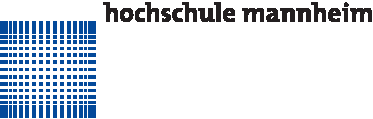
\includegraphics{logo.pdf}}
\end{textblock*}%
\begin{textblock*}{130mm}(48mm,68mm) % 4,8cm vom linken Rand und 6,8cmm vom oberen Rand
	\centering\huge\bfseries
	Virtualisierte Arbeitsumgebung für den Test verteilter Systeme
\end{textblock*}%

%Name
\begin{textblock*}{130mm}(48mm,105mm)
	\centering\Large\itshape 
	Jan-Philipp Willem
\end{textblock*}

%Rest
\begin{textblock*}{297mm}(-36mm,150mm) % -46mm muss vielleicht angepasst werden - von Bindungkorrektur abhängig
	\begin{center}
		{\scshape\Large Studienarbeit\\ Studiengang Informatik}\\
		\vspace{2cm}
		{\scshape\large Fakultät für Informatik\\Hochschule Mannheim}\\
		\vspace{2cm}
		{\large 23.06.2017} \\ %Datum
		\vspace{3,5cm}
		{\large Betreuer: Prof. Dr. Sandro Leuchter\\
		Zweitkorrektor: Prof. ...}
	\end{center}
\end{textblock*}
\end{titlepage}
\null
\newpage

  % \begin{titlepage}
{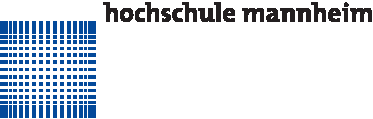
\includegraphics{logo.pdf}}\par
\vspace{4cm}
% \centering
{\scshape\LARGE Fakultät für Informatik \par Hochschule Mannheim\par}
\vspace{0.66cm}
{\scshape\Large Studienarbeit\par}
\vspace{.033cm}
{\huge\bfseries Virtualisierte Arbeitsumgebung\par für den Test verteilter Systeme\par}
{\LARGE Microservice-Architektur mit Docker,\par Clojure \& Elm\par}
\vspace{0.66cm}
{\Large\itshape Jan-Philipp Willem ---}
\vspace{.1cm}
{\Large 23.06.2017}
\vfill
\end{titlepage}

  \begin{abstract}
  Ein verteiltes Softwaresystem zu entwickeln und ebenso dessen Auswirkungen zu verstehen, ist kein Leichtes für einen durchschnittlichen Informatik-Studenten.
  Oft ist es der Fall, dass es schon anspruchsvoll genug ist, alleine die Grundlagen umzusetzen, welche es bei einer Aufgabe anzuwenden vermag. 
  Um diese Hürde etwas zu erleichtern, soll eine Umgebung geschaffen werden, welche es ermöglicht, eine verteilte Aufgabe unabhängig des eigenen Computers zu testen.
  Eine Programmieraufgabe soll von einem Dozenten als ein Experiment definiert werden können, welches aus einer gegebene Anzahl an Instanzen eines ebenso definierten Servers-Systems besteht.
  Weiterhin soll das Experiment von einem Studenten durchgeführt werden können, welches das Hochladen der eigenen Lösung und das anschließende Analysieren der darin resultierenden Ausgaben der voneinander getrennten Rechner-Instanzen darstellt.
  \\\\\\
  \hspace*{.43\textwidth}\textbf{Abstract}
  \\\\
  \blindtext
\end{abstract}


  \pagenumbering{roman}
  \setcounter{page}{3}
  
  \tableofcontents
  \listoffigures
  % \listoftables
  \clearpage

  \pagenumbering{arabic}

  \chapter{Problemstellung}
[Introduction] \blindtext
\section{Bisheriger Ablauf}
Der typische Ablauf bei Programmieraufgaben in der Vorlesung \ac{VAR} ist folgendermaßen:
Ein Student soll verteilte Aufgaben programmieren, welche es nötig machen, zunächst eine passende lokale Entwicklungsumgebung zu installieren.
Dazu wird die Nutzung von schwergewichtigen \acp{IDE} wie Eclipse oder Netbeans vorgeschlagen.
Grund dafür sind die schon vorhandenen \ac{IDE}-Integrationen von diversen Serven und Technologien, welche eingesetzt werden sollen.
Dennoch führt schon dieser Prozess bei einigen Studenten zu Problemen.
\par
Gelingt es die Integrationen einzurichten, so kann die Funktionsweise der eigenen Programme getestet werden.
Allerdings führt diese Herangehensweise zu keiner echten Verteilung, da alle Services auf der gleichen Maschine ausgeführt werden.
Das Ergebnis kann sich bei einer Trennung der Services auf Netzwerkebene erheblich unterscheiden oder ist unter Umständen gar nicht lauffähig.
\par
[TODO: Beispiel einer Aufgabe z.B. RMI-Chat]
\section{Anforderungen}
Ziel soll es sein, dass ein Dozent Experimente definieren kann, welche eine gegebene Anzahl an Instanzen besitzen.
Eine jeweilige Instanz wird durch die Angabe eines Namens, dessen geöffneten Netzwerk-Ports und eine Argumentenliste beschrieben.
Die Konfiguration der Systeme soll mit Hilfe eines Dockerfiles realisiert werden.
Die Instanzen sollen sich gegenseitig erreichen können, jedoch soll der Zugriff auf Instanzen anderer Nutzer und dem Internet unterbunden werden.
\par
Weiterhin sollen von einem Studenten gewisse Aufgaben innerhalb dieser Experimente gelöst werden.
Dies geschieht durch einzelnes Hochladen der Programmpakete (Jar, War,..) pro Instanz und der Angabe einer Main-Class und einer Argumentenliste.
Anschließend kann eine Instanz gestartet werden und dessen Ausgaben beobachtet werden.
\par
Der Grund für das getrennte Hochladen ist darin begründet, dass die echte Verteilung der Instanzen so von den Studenten eventuell besser verstanden werden kann.


  \chapter{Grundlagen}
\label{ch:fundamentals}

Dieses Kapitel möchte einige Grundlagen definieren, welche im Kapitel~\ref{ch:main-matter} vorausgesetzt werden.
Es handelt von der Definition des funktionalen Programmier-Paradigma, welches in den Sprachen Clojure und Elm zum Einsatz kommt.
Weiterhin werden die Webtechnologien Websockets und \acp{SPA} erklärt, welche das Frontend des \nameref{ch:main-matter}'s nutzt. 
Die Architektur der ganzen Applikation wird maßgebend durch die Trennung in unabhängige Microservices beeinflusst, welche mit Docker realisiert sind.
\section{Funktionale Programmierung}
Die funktionale Programmierung gehört zu den Deklarativen Programmierparadigmen und stellt neben der imperativen und objektorientierten Programmierung eines der am Häufigsten genutzten Paradigmen dar.
\par
Anders als bei imperativen Sprachen, unterscheiden sich funktionale Sprachen vor Allem an ihrer Unveränderbarkeit (engl. Immutability) von Variablen und ihrer Datenstrukturen.
Es wird dabei angestrebt, bei einer Veränderung des Zustandes einer Variablen nicht den Inhalt ihrer Referenz zu verändern, sondern stattdessen eine Kopie der Daten zurückzuliefern.
In der Praxis(TODO: quote) hat sich vielfach herausgestellt, dass sich die häufig verwendete Veränderbarkeit (engl. Mutability) von Zuständen gerade auch in der objektorientierten Programmierung zu häufigen Fehlerquellen führen kann.
Es wurde jedoch gezeigt, dass das Zurückgeben von Kopien ebenso sehr performant funktionieren kann (TODO: add quote).
\par
Wie der Name schon vermuten lässt basiert die funktionale Programmierung zu größten Teilen aus Funktionen. 
Diese sind meist als Module gekapselt, welche nach einer bestimmten Aufgabe gruppiert sind. 
Anders als bei Objekten möchte man offen mit den an die Funktionen übergebenen Daten umgehen und sie nicht in der Implementierung verstecken (engl. Information-Hiding). 
Dabei sollte eine Funktion nur diese eine Aufgabe erledigen, welche mithilfe ihres Namens beschrieben wird. 
Um dieses deterministische Verhalten zu erreichen, werden oft sehr granulare Funktionen erstellt, welche anschließend durch eine Komposition miteinander vereint werden\footnote{\texttt{f(x) = g(x) • h(x) <=> f(x) = h(g(x))}}.
Jegliche Seiteneffekte sollten vermieden werden, was man auch als reine (engl. pure) Funktionen bezeichnet.
So sollten Funktionen als Daten-Transformationen verstanden werden: Man erhält Daten, verarbeitet diese und gibt sie anschließend transformiert zurück, welches als \ac{EVA}-Prinzip bekannt ist.
\par
Da Funktionen selbst auch Typen darstellen, können sie ebenso als Parameter anderer Funktionen dienen, welche man dann auch als Funktionen Höherer Ordnung (engl. Higher Order Funktions) bezeichnet.
Mit dieser Voraussetzung können Verhalten aus einer aufzurufenden Funktion herausgelöst werden, womit das jeweilige Verhalten dynamisch bestimmt werden kann.
Dies wird oft auch als Callbacks bezeichnet.
Hilfreich sind bei dieser Vorgehensweise auch so genannte Lamdas, welche Funktionen darstellen, die inline definiert werden können und somit anonym \ac{bzw.} Unbenannt sind.
\par
Grundsätzlich werden funktionale Sprachen nochmals zwischen solchen Sprachen unterschieden, welche neben anderen Paradigmen auch das Funktionale Paradigma unterstützen und solchen, welche ausschließlich auf den Prinzipien der funktionalen Programmierung beruhen.
Die sogenannten reinen funktionalen Sprachen verbieten \ac{bspw.} eine jegliche Möglichkeit Seiteneffekte auszuführen und sind sehr oft strikt typisiert.
In Multiparadigmensprachen beruhen viele funktionale Prinzipien auf deren Einsatz und der generellen Bedachtheit des jeweiligen Programmierers \ac{bzw.} des einsetzenden Teams.

\section{Verwendete Programmiersprachen}
Das Projekt verwendet für den Server die Sprache Clojure, wohingegen der Client mithilfe von Elm umgesetzt ist.
\subsection{Clojure}
\blindtext
\par
\blindtext
\subsection{Elm}
\blindtext
\par
\blindtext
\section{Eingesetzte Webtechnologien}
\subsection{Websockets}
\blindtext
\subsection{\aclp{SPA}}
\blindtext
\section{Container-Virtualisierung mit Docker}
\begin{figure}
  \centering
  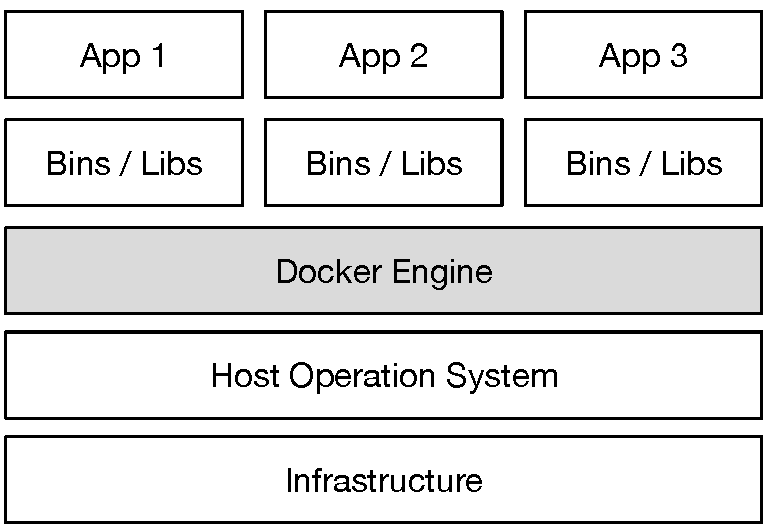
\includegraphics[scale=0.75]{docker.pdf}
  \par
  \caption{Schichten einer Virtualisierung mit Docker}
  \label{fig:layers-docker}
\end{figure}
Docker\footnote{\url{https://docs.docker.com/}} ist eine Software zum Deployment von Applikationen innerhalb von Containern.
Im Vergleich zu \acp{VM}, ähnelt sich die Vorgehensweise, jedoch laufen die Prozesse der Container direkt auf dem Host-Betriebssystem.
Trotz dieser Tatsache sind die Prozesse mithilfe von \ac{u.A.} Control-Groups und Kernel Namespaces voneinander isoliert.
Weiterhin hat man die Möglichkeit mit gängigen Mandatory-Access-Control-Frameworks wie SE-Linux oder App-Armor die Rechte innerhalb der Container zu beschränken.
Als Anforderung besteht keine spezifische Hardware-Infrastruktur wie bei beispielsweise VMWare ESXi.
Ebenso ist Docker mittlerweile auf allen gängigen Betriebssystemen lauffähig, wobei Linux-Derivate die beste Unterstützung erhalten.
Dies ist damit begründet, dass die Docker-Engine (\acs{Abb.}~\ref{fig:layers-docker}) auf den einzelnen Betriebssystemen verschieden aussieht.
\par
Ein Container wird mithilfe eines Dockerfiles beschrieben.
Darin werden deskriptive Instruktionen definiert um Abhängigkeiten zu installieren, Konfigurationen vorzunehmen und andere Build-Steps auszuführen.
Ein spezifischer Container wird als Image bezeichnet und setzt sich aus granularen Sub-Images zusammen.
Beim Erzeugen von Images eigener Dockerfiles müssen im Vergleich zu \acp{VM} keine großen Dateien transferiert werden, da sie aus ihrem Rezept reproduzierbar sind. 
Es besteht auch die Möglichkeit, von anderen Dockerfiles zu erben und diese über das Netzwerk verteilt bereitzustellen.
Falls die über eine Docker-Registry angebotenen Schichten eines Containers noch nicht auf dem eigenen Rechner vorhanden sind, so werden diese heruntergeladen.
\par
Weiterhin gibt es einen entscheidenden Vorteil gegenüber einer traditionellen \ac{VM}: Ein Dockerfile trägt implizit zur Dokumentation bei, da jede Änderung an einem Container in seinem Rezept ergänzt werden muss, um diese bei einem erneuten Start \ac{bzw.} erneuten Build zu erhalten.
\par
Wird eine Applikation in einzelnen Services aufgeteilt, so bietet sich das Tool \textbf{Docker-Compose}\footnote{\url{https://docs.docker.com/compose/overview/}} an.
Es ermöglicht in einer einzelnen Datei (\texttt{docker-\break compose.yml}) alle Konfigurations-Parameter der einzelnen Containern zu definieren.
Das können \ac{bspw.} Volume-Mounts, Ports, Environment-Variables oder Netzwerke sein, welche sonst bei jedem \texttt{docker exec} Command angegeben werden müssten.
Alternativ dazu stünden eigene und oft fehlerintensive Shell-Scripts um ähnliches zu erreichen. 
\par
Es bietet sich auch an, getrennte Environments für Development, Test und Production als zentrale Dokumentation der Applikation zu nutzen (\texttt{docker-\break compose.[env].yml}).


  \chapter{VAR-Tool}
\label{ch:main-matter}
  \begin{figure}[H]
    \centering
    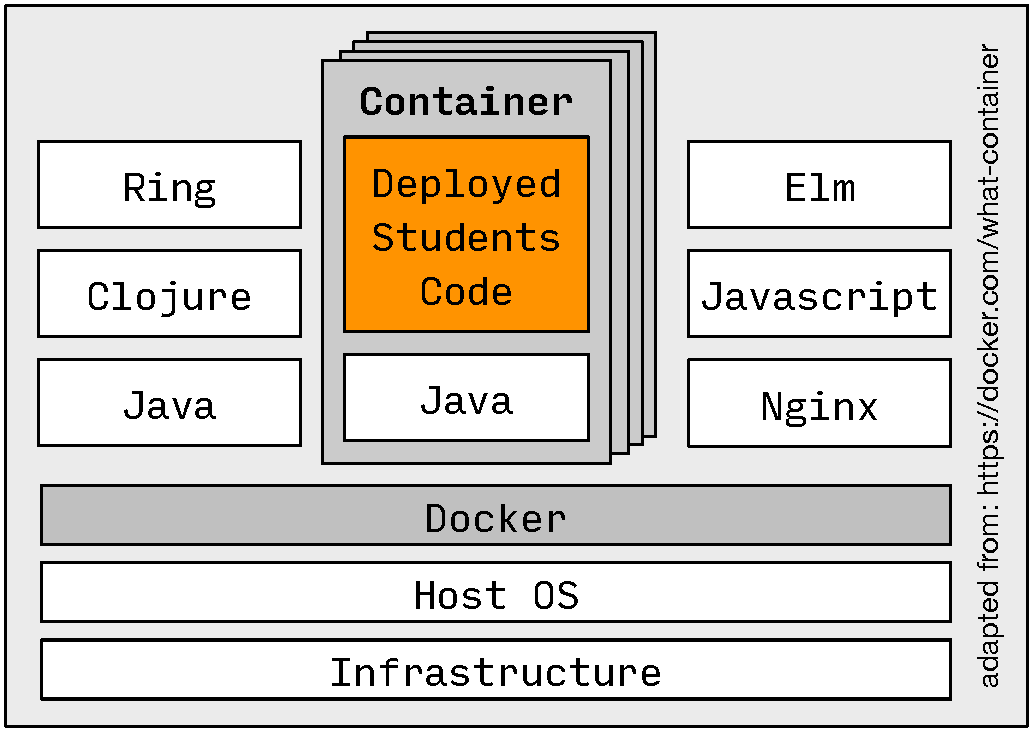
\includegraphics[scale=0.4]{container_intro_centered.pdf}
    \par
    \caption{Container-Übersicht}
    \label{fig:container-intro}
  \end{figure}
  Diese Kapitel beschreibt die Vorgehensweise und Umsetzung des VAR-Tools.
  Es wird zunächst ein Mockup des Clients vorgestellt und dann auf die weitere Architektur des Systems eigegangen.
  Abbildung~\ref{fig:container-intro} zeigt eine Übersicht der geplanten Applikation.
  Wir haben auf der linken Seite einen Server-Container, welcher auf Java bzw. Clojure aufgebaut ist.
  Daneben befinden sich mehrere User-Container in denen anschließend Programmpakete eines Studierenden ausgeliefert werden sollen.
  Auf der rechten Seite ist ein Client-Container sichtbar, welcher aus einem Webserver (Nginx) besteht.
  Dieser liefert eine statische HTML-Seite aus, in welcher eine Elm-Applikation als Java-Script integriert ist.
  Die Container laufen auf einem Rechner, auf dem Docker installiert ist und aus einer beliebigen Infrastruktur besteht.
  \clearpage

% \section{Analyse}
% \subsection{As-Is}
% \subsection{To-Be}

\section{UI-Mockup}
Im Vorfeld wurde überlegt, welche Features ein Client zur Darstellung von Instanzlogs besitzen soll.
Dazu wurden Skizzen auf dem Papier entwickelt, bevor es dazu kommen sollte, ein einfach gehaltenes Design einer Oberfläche zu gestalten.
\par
Abbildung~\ref{fig:ui-mockup-1} zeigt eine Übersichtsseite, welche die verfügbaren Experimente als anklickbare Quadrate mit einem beschreibenden Titel darstellt.
Auf der linken Seite könnte eine Menüleiste enstehen, welche die benötigten Aktionen bereitstellt.
So gibt es darin ein Link zu der Experimentenübersicht und eine Verlinkung zu einer Hilfe bzw. dem Autor des Tools.
\par
Bei einem Öffnen eines Experiments sollen wie in Abbildung~\ref{fig:ui-mockup-2} eine gewisse Anzahl an zugehörigen Instanzen dargestellt werden.
Diese Instanzen können verschiedene Zustände aufweisen.
\par
Der erste Zustand wird in der unteren Ecke skizziert und erlaubt eine Dateiauswahl um ein Programmpaket hochzuladen.
Bei einem Drag-and-Drop einer Datei auf der Instanz soll es ebenso möglich sein, diese zum Hochladen anzunehmen.
\par
Die rechte untere Ecke zeigt eine Instanz, welche auf weitere Ereignisse von dem Server wartet.
Es wird ein beschreibender Text und ein drehendes Warte-Icon dargestellt.
Dieser Zustand soll bei einem Hochladen und auch bei einem Instanzstart angezeigt werden.
\par
Der nächste Zustand (oben links) ermöglicht es, der zu startenden Instanz, eine Hauptklasse innerhalb des Programmpakets und eine Argumentenliste zu übergeben.
Ebenso wird in einem Schaubild visualisiert, welche Ports an der Instanz geöffnet sind.
Diese sind nicht zu bearbeiten, sollen aber nochmals auf die Aufgabenbeschreibung erinnern.
Die hochgeladene Datei wird mit ihrem Namen dargestellt und man kann diese auch wieder mit dem Mülleimer-Icon löschen.
Daraufhin wird wieder der Upload-Zustand gezeigt.
\par
Die rechte obere Ecke zeigt eine Instanz, welche gestartet wurde und stellt darin geschehene Ausgaben dar.
Man kann die Instanz mit einem Stop-Icon anhalten.
\begin{landscape}
  \begin{figure}[h]
    \centering
    \fbox{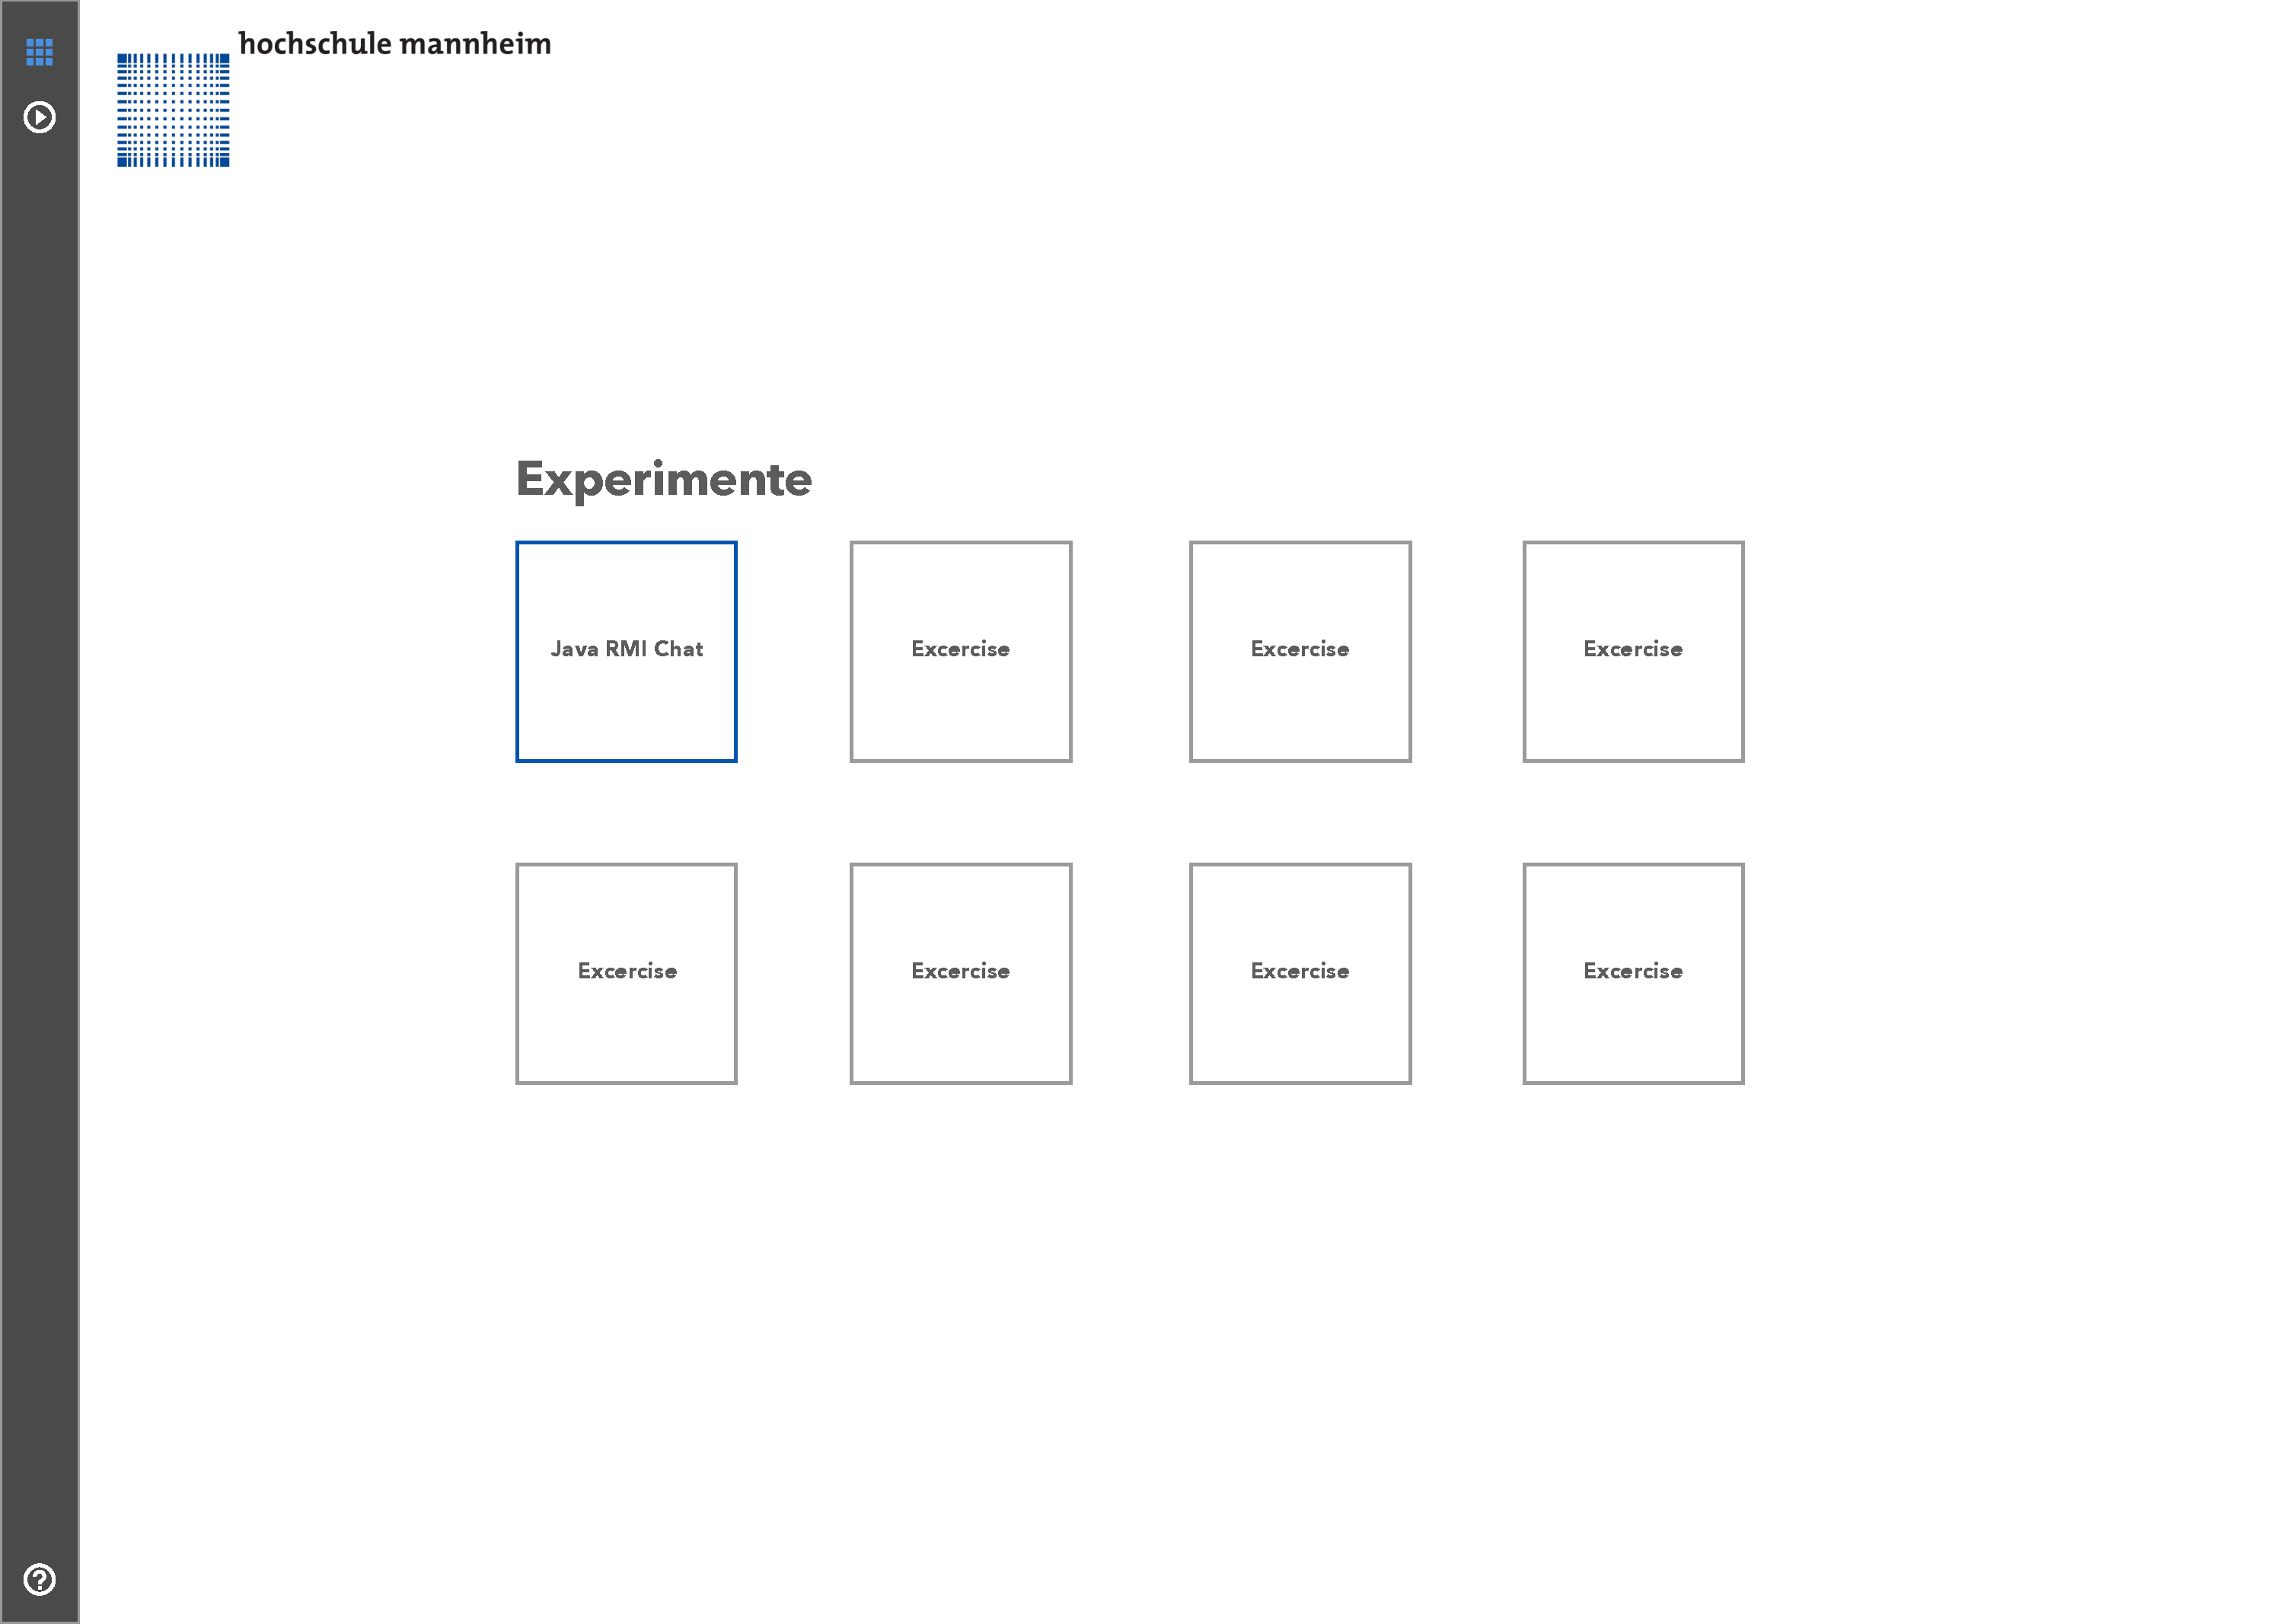
\includegraphics[scale=0.4,page=1]{ui-mockup.pdf}}
    \par
    \caption{UI-Mockup: Übersicht der Experimente}
    \label{fig:ui-mockup-1}
  \end{figure}
  \begin{figure}[h]
    \centering
    \fbox{\includegraphics[scale=0.4,page=2]{ui-mockup.pdf}}
    \par
    \caption{UI-Mockup: Experimentenansicht mit verschiedenen Zuständen pro Instanz}
    \label{fig:ui-mockup-2}
  \end{figure}
\end{landscape}

\section{Architektur}
% Dieses Kapitel
\subsection{User-Stories}
Aufgrund seiner Eignung bei agilen Entwicklungsmethoden wurden User-Stories ausgewählt, um als kompakte Beschreibungen der Anforderungen der Applikation zu dienen.
Das folgende Schema dient dabei als Vorlage: \\\textit{„Als \{Rolle\} möchte ich \{Ziel/Wunsch\}, um \{Nutzen\}.“}
\begin{enumerate}
  \item Als Studierender möchte ich ein Experiment aus einer Liste auswählen, um dieses durchführen zu können.
  \item Als Studierender möchte ich ein Programmpaket hochladen können, damit ich meine Lösung einer Aufgabe in einer eigenen Instanz testen kann.
  \item Als Studierender möchte ich Änderungen an den Parametern einer Instanz vornehmen können, damit ich den Ablauf meines Programms bewusst von außen beeinflussen kann.
  \item Als Studierender möchte ich eine Instanz meines Programms starten können, um diese mit anderen unabhängigen Instanzen interagieren zu lassen.
  \item Als Studierender möchte ich die Standard-Ausgaben einer laufenden Instanz meines Programms von außen aktiv verfolgen können, damit ich dessen Verhalten analysieren kann.
  \item Als Studierender möchte ich die Standard-Eingaben einer laufenden Instanz von außen aktiv beeinflussen können, damit ich Eingaben in meinem Programm nutzen kann.
  \item Als Studierender möchte ich eine laufende Instanz anhalten und dessen geladenes Programmpaket zurücksetzen können.
\end{enumerate}
Abbildung \ref{fig:state} zeigt ein Zustandsdiagramm um den Ablauf der Applikation mit seinen einzelnen Features abzubilden.
Ein Studierender beginnt, indem er die URL des VAR-Tools in seinem Browser eingibt.
Dies hat ein Request des Browsers an den Client zur Folge, woraufhin der Browser die Dateien \texttt{index.html} und \texttt{main.js} erhält.
Bei Durchführung der ersten User-Story, gelangt ein Studierender zu einem Experiment, welches Instanzen enthält.
Eine Instanz hat vier verschiedene Zustände: Empty, Waiting, Settings und Running.
Wird die zweite User-Story angewendet, ändert sich der Zustand der jeweiligen Instanz auf Waiting mit dem Kind-Zustand von Uploading.
Im Hintergrund sendet die Applikation einen Request an den Server um das ausgewählte Programmpaket hochzuladen.
Wird eine Antwort erhalten, so wird der Zustand der Instanz auf Settings gesetzt.
Die Instanz-Parameter im Zustand Settings erfüllen User-Story drei und vier.
Außerdem kann in diesem Zustand das geladene Programmpaket gelöscht werden (User-Story sieben).
Wird der Button zum Starten einer Instanz ausgewählt, so wird der Zustand auf Waiting gesetzt, wobei diesmal ein Hinweis auf das Starten angezeigt werden soll (Kind-Zustand von Starting).
Der Browser sendet eine Anfrage um die jeweilige Instanz zu starten.
Bei einem Start wird die Instanz mit den Eingaben aus den Instanz-Parametern im Server  vorbereitet und als ein User-Container mit Docker gestartet.
Nachdem die Applikation im Browser ein Signal des Servers von einem Start der Instanz erhält, wird dort der Zustand Running angezeigt.
In diesem Zustand ist es möglich, User-Story fünf und sechs anzuwenden.
D.h. die Ausgaben aus der laufenden Instanz werden kontinuierlich dargestellt und es ist möglich Eingaben zu machen.
Weiterhin kann dort der andere Teil der User-Story sieben zum Tragen kommen, was ein Anhalten des User-Containers der Instanz auf dem Host zur Folge hat.



\begin{landscape}
  \begin{figure}[h]
    \centering
    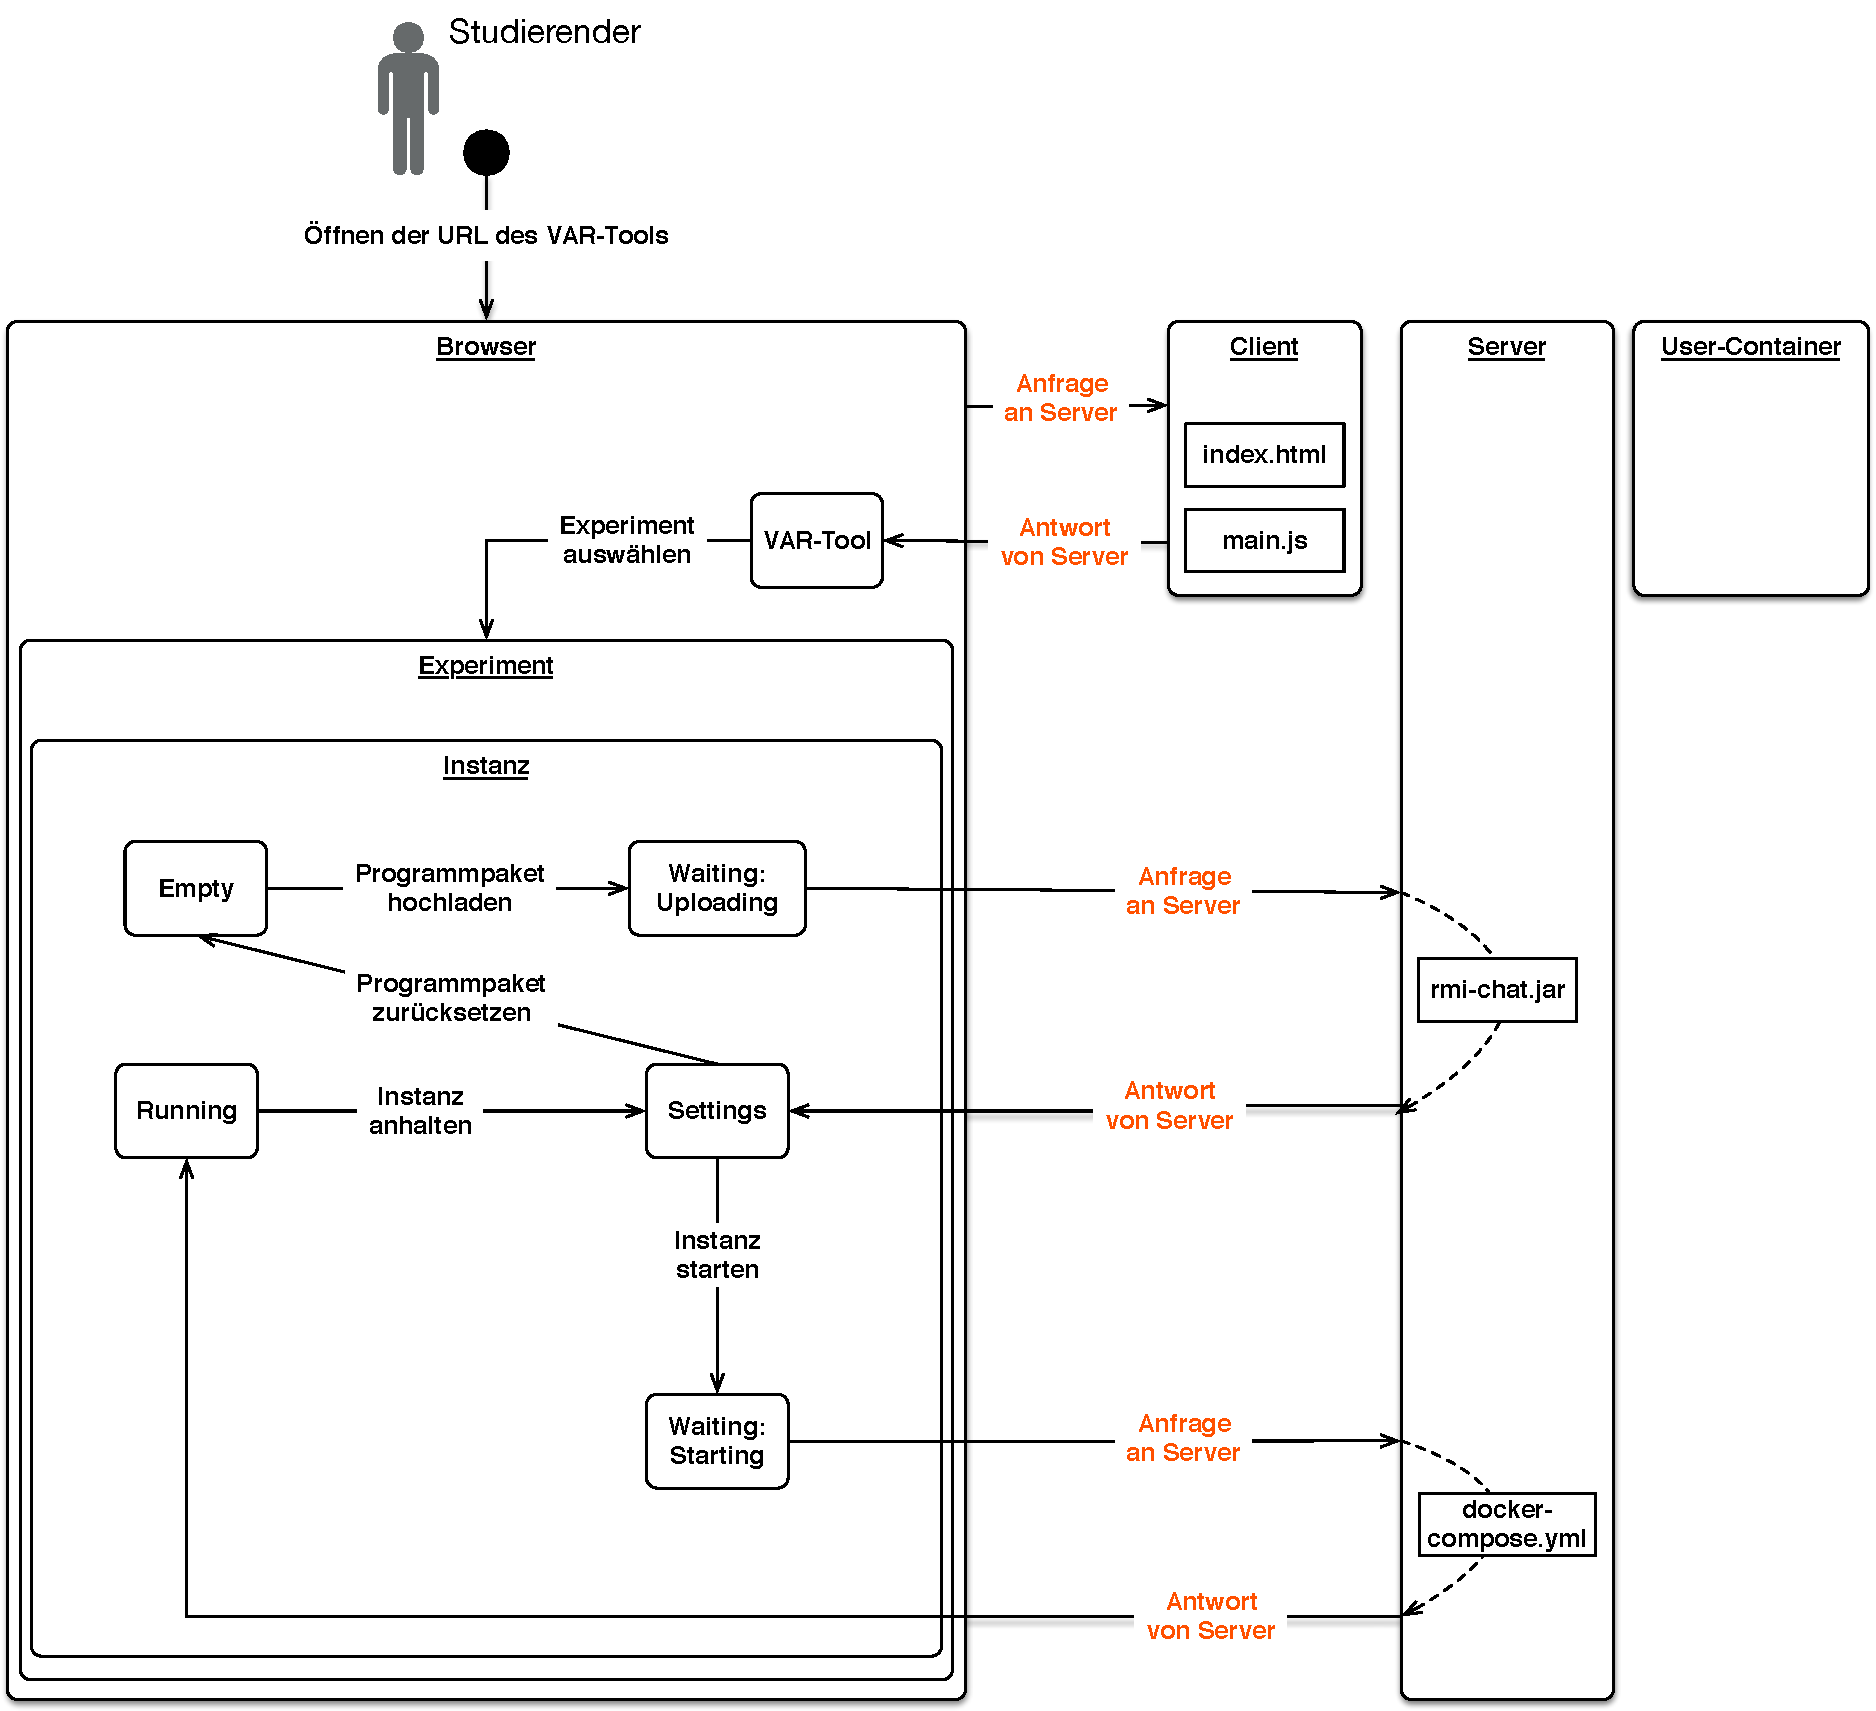
\includegraphics[scale=0.5]{states.pdf}
    \par
    \caption{Zustandsdiagramm}
    \label{fig:state}
  \end{figure}
\end{landscape}

\subsection{Netzwerkgrenzen}
  \begin{figure}[h]
    \centering
    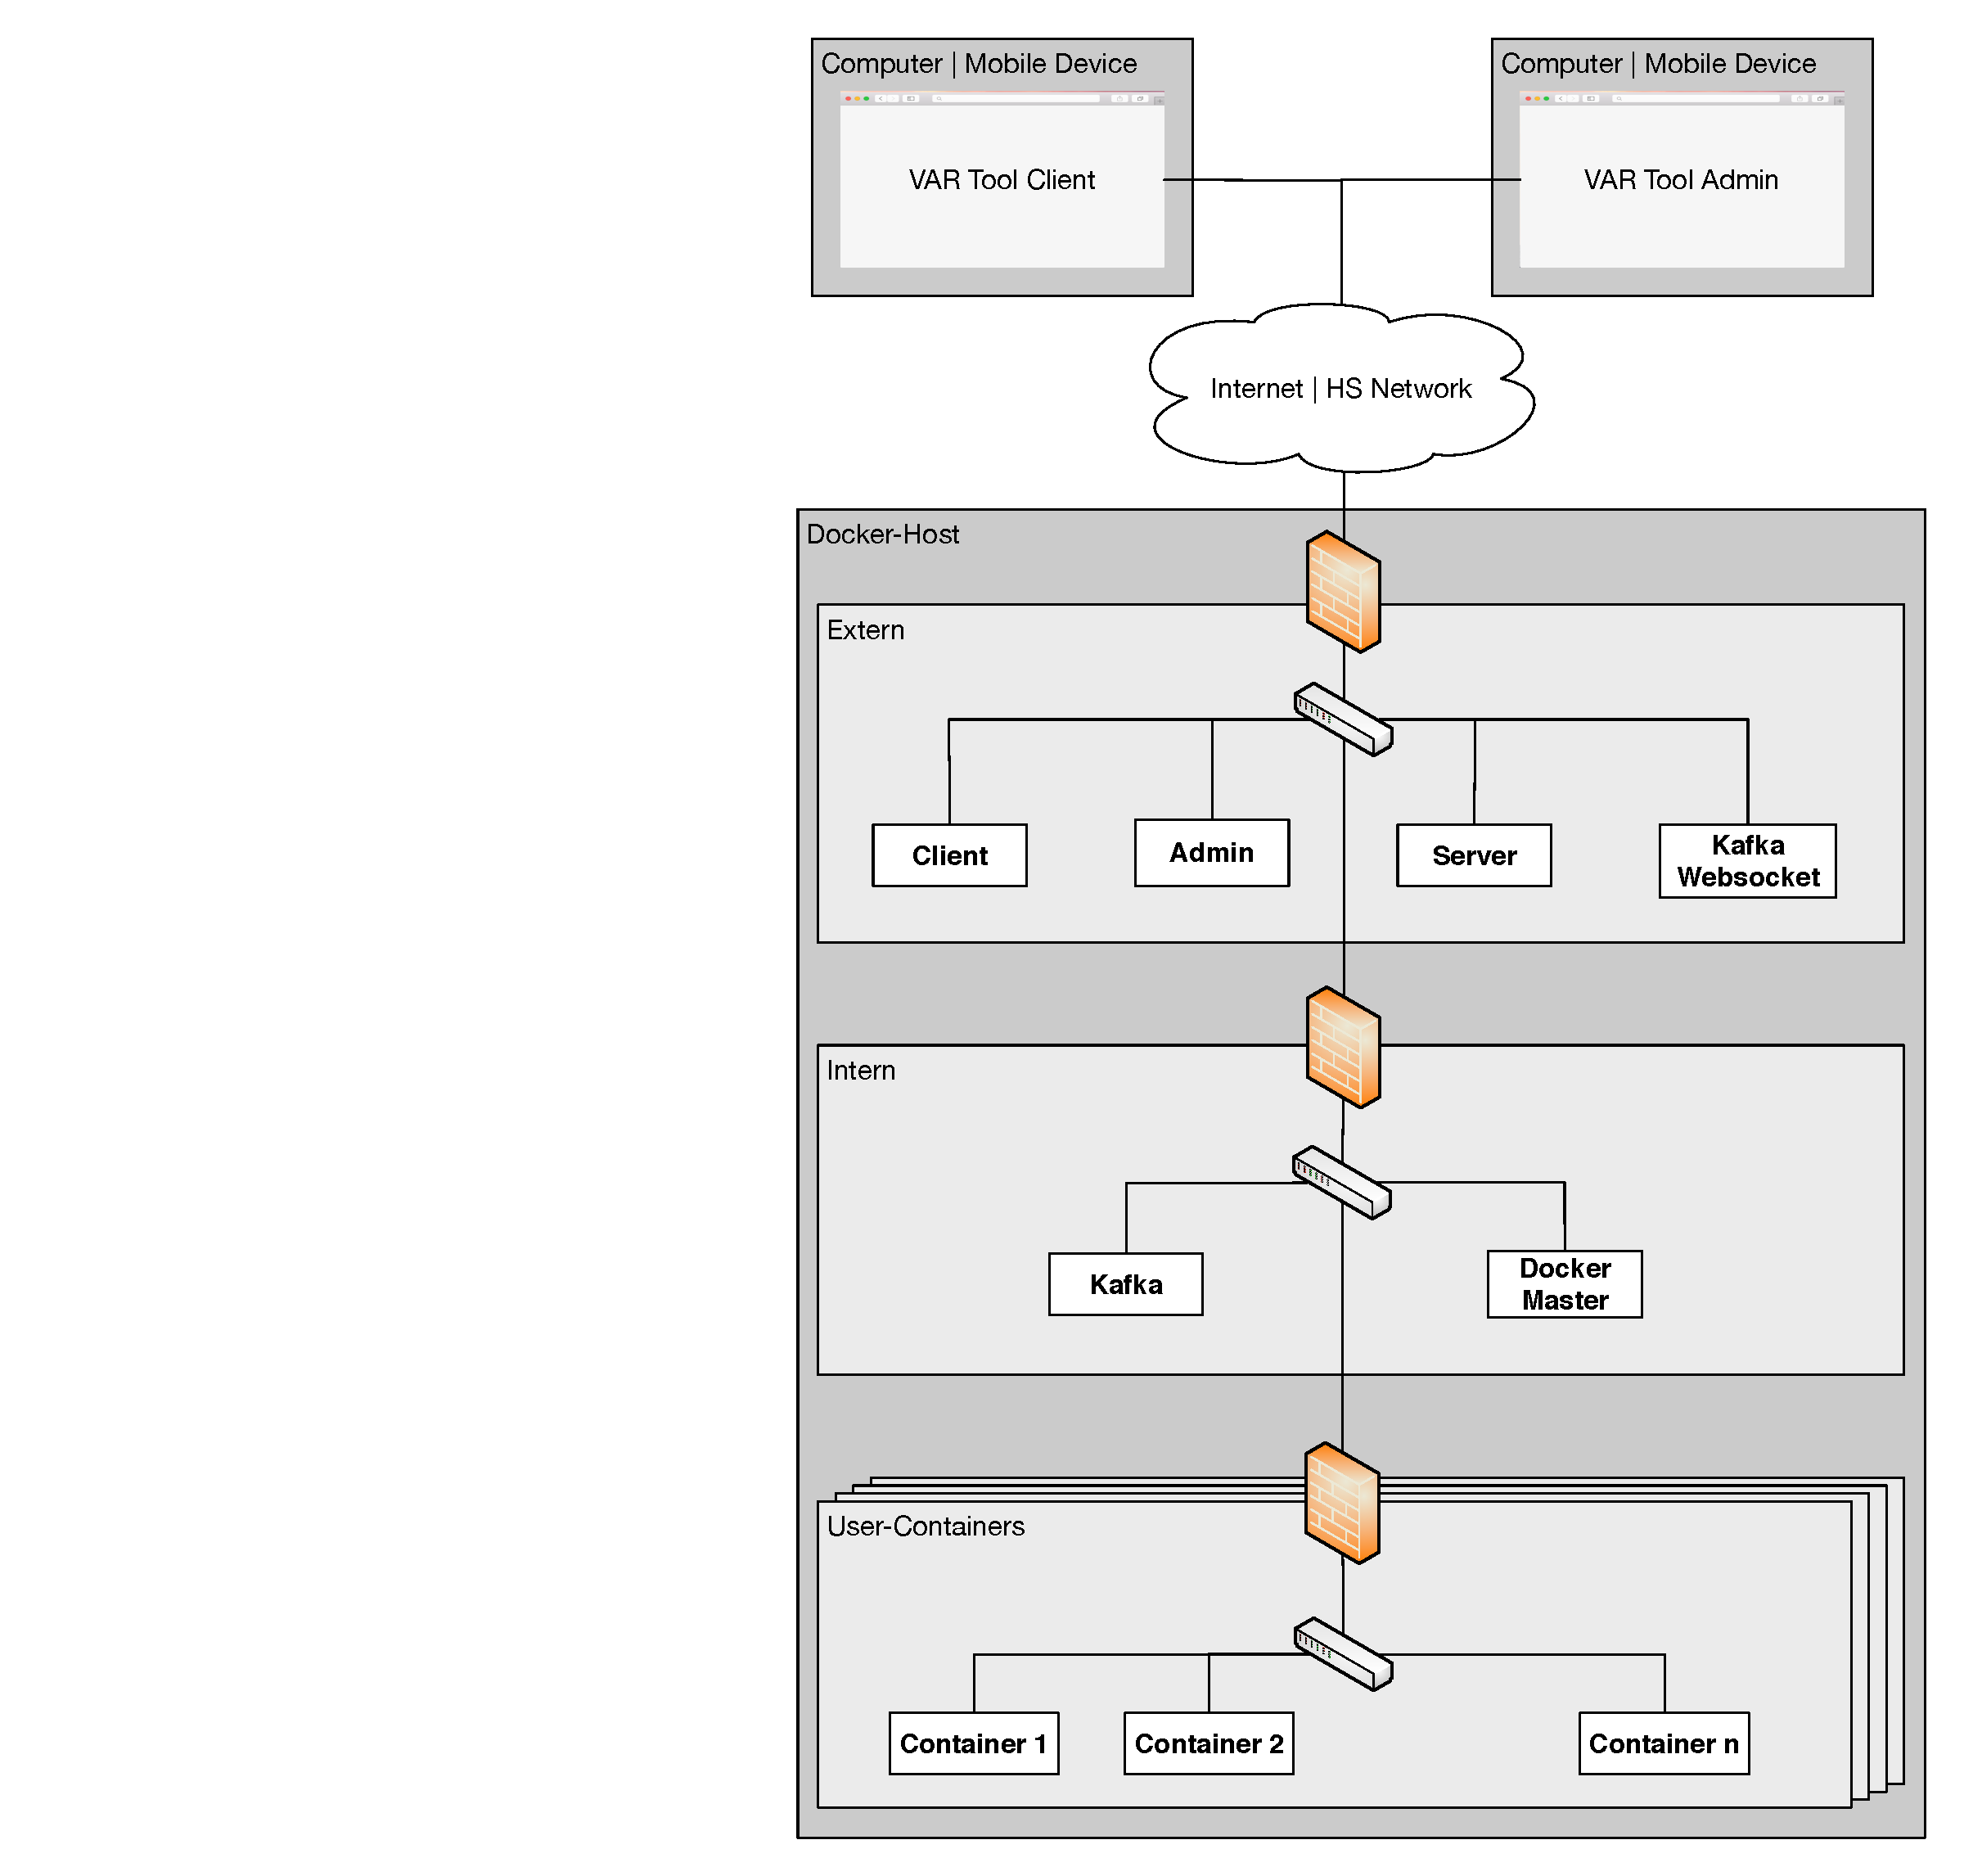
\includegraphics[scale=0.5]{network.pdf}
    % \par
    \caption{Netzwerkdiagramm}
    \label{fig:network}
  \end{figure}
  
Es wird ein Rechner benötigt, welcher aus dem Internet oder hochschulintern erreichbar ist.
  Auf diesem läuft Docker und stellt die Applikation des Projekts bereit.
  Die Zahl an Benutzern des Clients und Admin-Clients ist beliebig, da das Frontend als Web-Applikation realisiert wird.
  \par
  Innerhalb von Docker existieren mehrere gekapselte Netzwerke, welche an einem Bridge-Interface des Docker-Hosts angeschlossen sind.
  Es werden nur solche Ports an den Netzwerken geöffnet, welche in einem Container freigegeben werden.
  Eines dieser Netzwerke stellt die eigentliche Applikation selbst dar und trägt den Namen \textit{vartool\_extern}.
  Ruft ein Studierender das VAR-Tool auf und startet darin eine Instanz eines Experiments, so wird ein neues Netzwerk angelegt.
  Dieses Netzwerk ist unabhängig von anderen Experimenten des gleichen und verschiedenen Studierenden, mit dem Namen \textit{vartool\_\{sessionToken\}\_\{experimentId\}}. 


\subsection{Deployment}
Abbildung~\ref{fig:deployment} zeigt die Verteilung der einzelnen Bestandteile der Applikation.
Die Container Server, User und die Clients werden mithilfe von Docker auf einem Linux-Rechner deployed.
\par
Der Client und Admin-Client bestehen jeweils aus dem Webserver \textit{nginx}, welcher ein statisches HTML-Dokument und ein Java-Script Bundle ausliefert, welches aus einer kompilierten Elm-Applikation resultiert.
Wird die URL eines Clients von einem beliebigen Rechner mit aktuellem Browser aufgerufen, so werden die benötigten Dateien übertragen und die Elm-App gestartet.
Während der Laufzeit des Clients verbindet sich der jeweilige Browser mit dem Server über einen Websocket.
Programmpakete welche hochgeladen werden sollen, werden über REST übertragen.
Es können dort anschließend verschiedene Experimente angezeigt und bei dessen Ausführung seine Ausgaben dargestellt werden.
Im Admin-Client sollen Statistiken dargestellt werden, welche u.A. die aktuelle Anzahl an experimentierenden Studierenden umfasst.
\par
Der Server besteht aus einer Java-Umgebung, welche ein Jar mit Clojure-Code ausführt.
Er hat die Aufgabe, einen Websocket-Endpoint anzubieten, welcher die Clients zur Kommunikation nutzen.
Ebenso soll dieser ein Endpoint anbieten, welcher ein Upload von Programmpaketen der Studierenden per POST-Request annimmt.
Jeder Benutzer bekommt einen temporären Ordner zugewiesen, in welchem seine Dateien gespeichert werden sollen.
Dieser User-Ordner werden anschließend für die zugewiesenen User-Container eines jeweiligen Studierenden verfügbar sein.
Mit diesem Seiteneffekt, über das File-System des Docker-Hosts, kann ein User-Container auf die jeweiligen Programmpakete zugreifen und diese ausführen.
\par
Ein solcher Container kann von dem Server gestartet werden, da der Server auf den Docker-Socket des Hosts zugreifen darf.
Sowohl die Eingaben wie auch resultierende Ausgaben sollen zunächst auch über das File-System zwischen Server und einzelnem User-Container geteilt werden.
Der Server reagiert auf die Änderung der Datei und schickt die Ausgaben an den Client.

\begin{landscape}
  \begin{figure}[h]
    \centering
    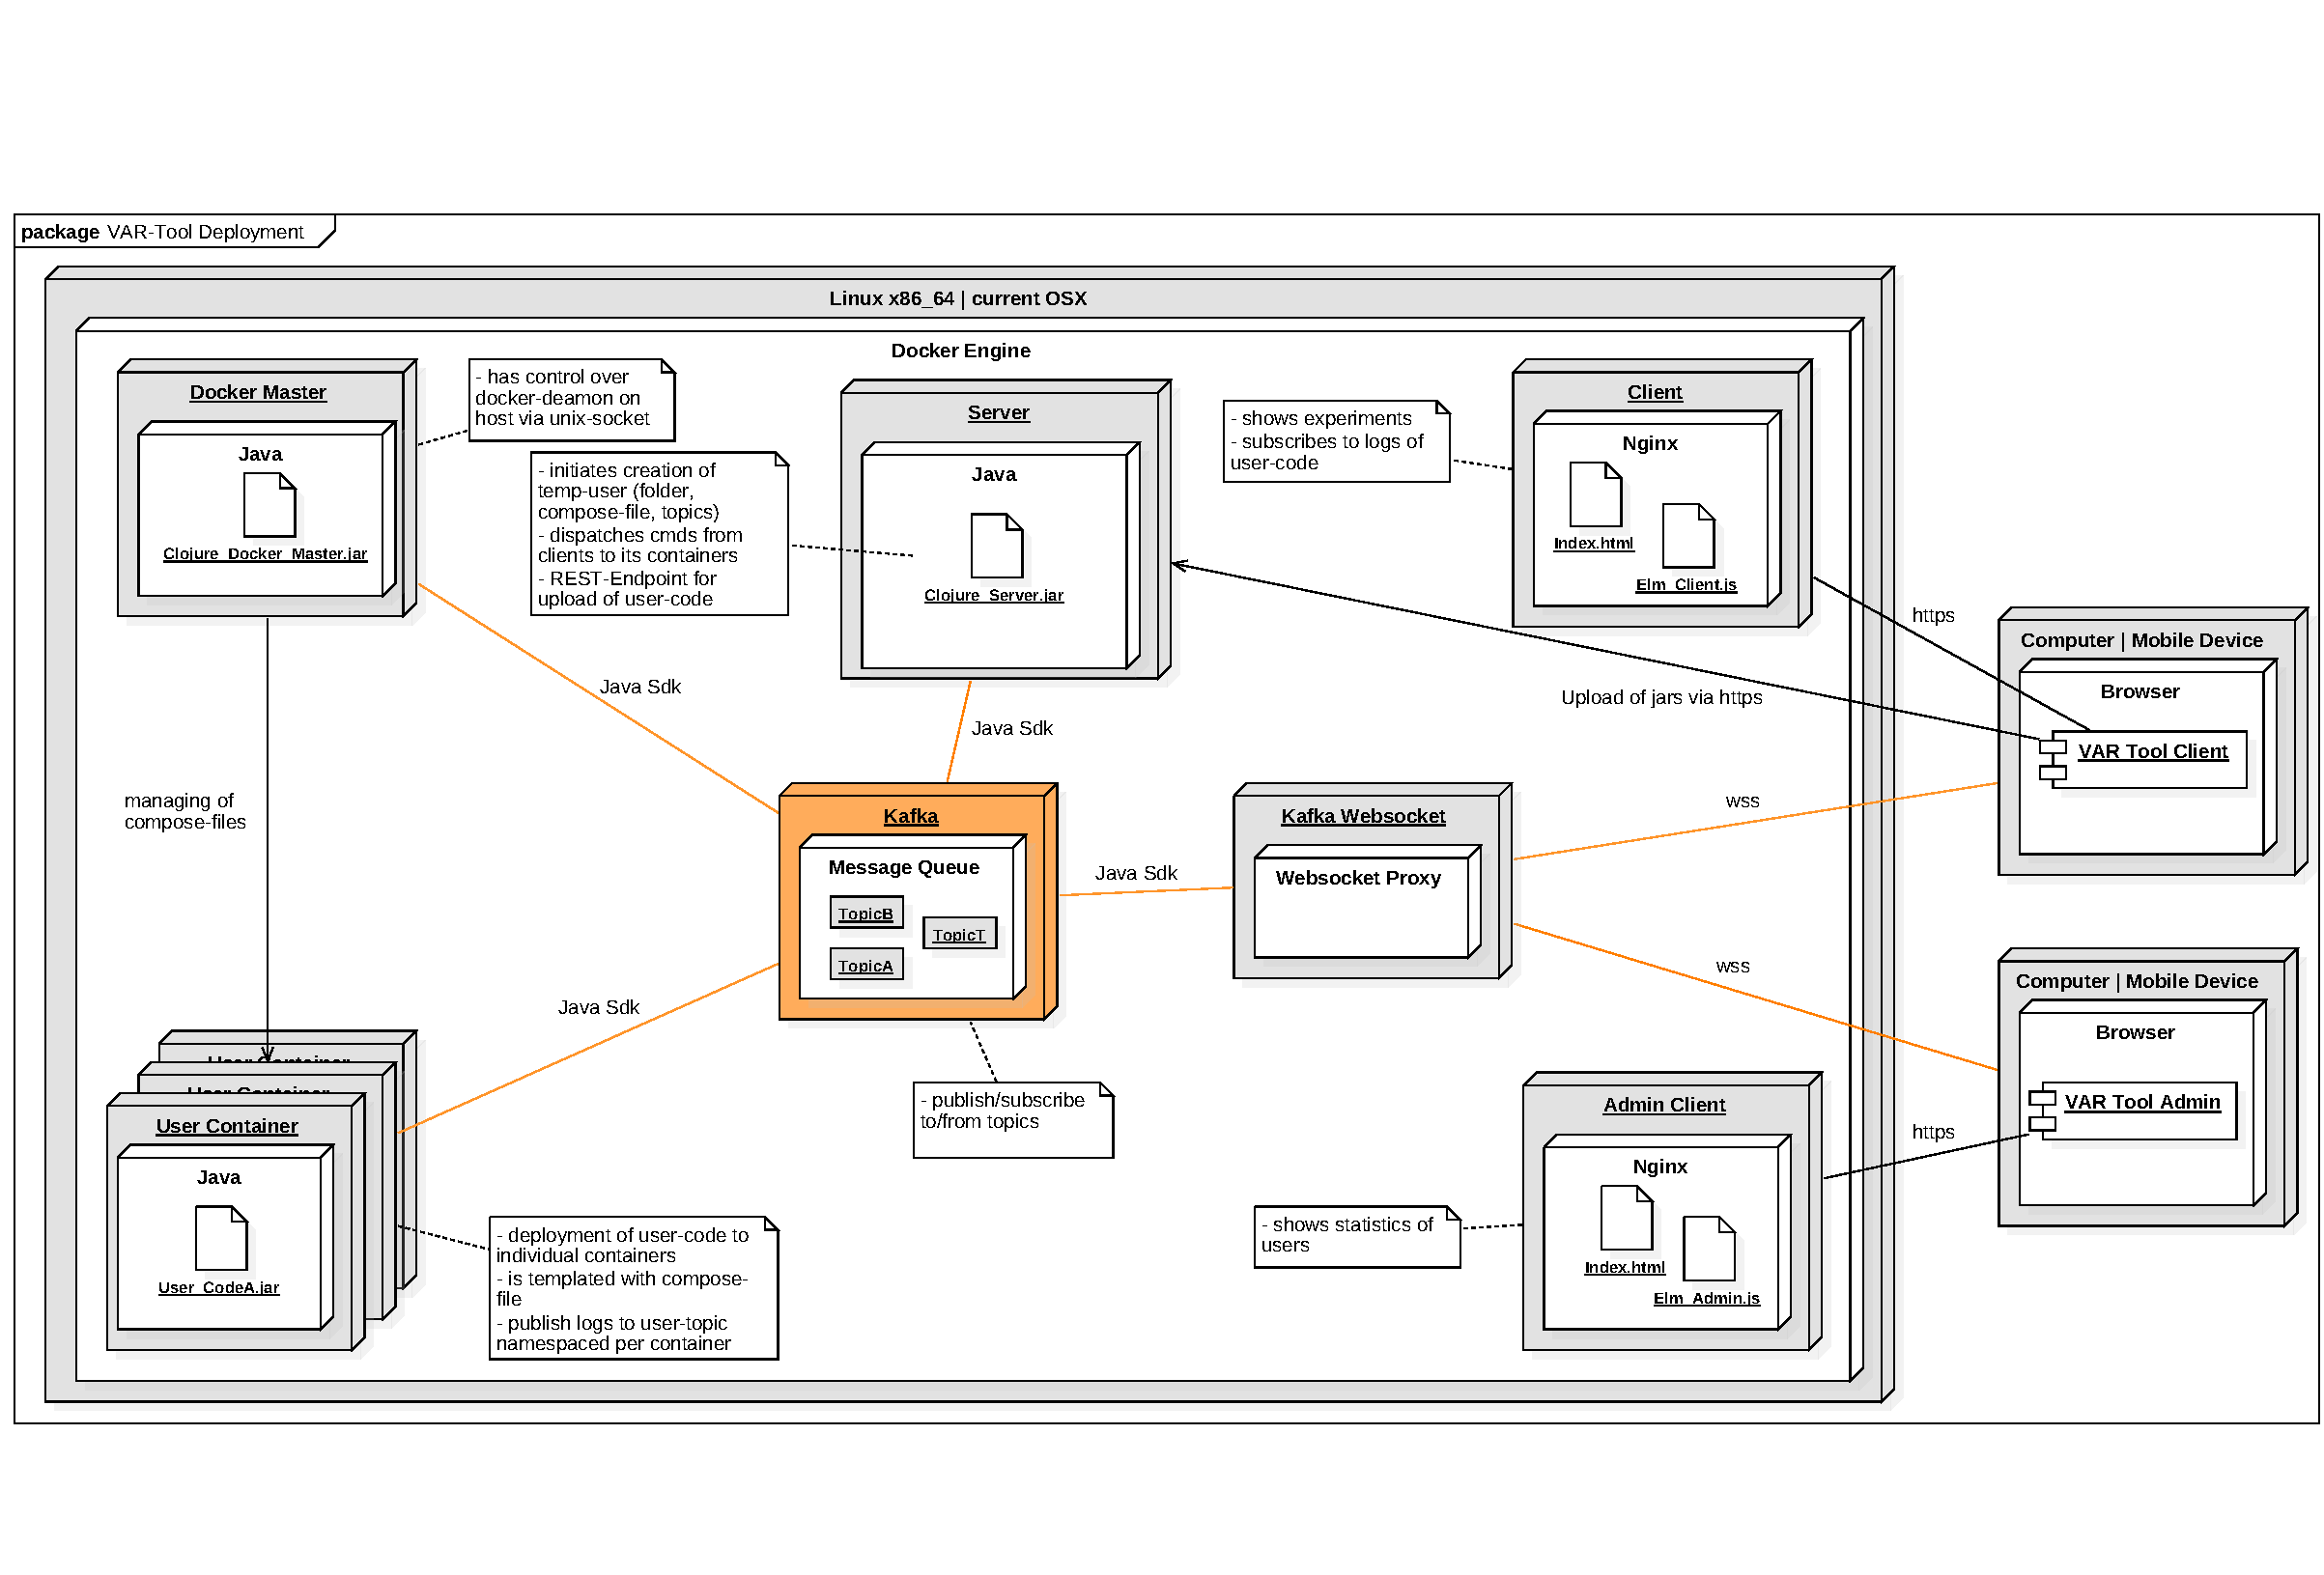
\includegraphics[scale=0.4]{deployment.pdf}
    \caption{Deploymentdiagramm}
    \label{fig:deployment}
  \end{figure}
\end{landscape}

\section{Umsetzung}
Im Folgenden werden Code-Beispiele gezeigt, welche in ihrem vollem Umfang im Repository des Projekts\footnote{\url{https://github.com/jwillem/var-tool}} zu finden sind.
\subsection{Kommunikation über Nachrichten}
Im Vorfeld wurde ein Nachrichten-Protokoll definiert, welches die Kommunikation zwischen Server und Client standardisiert.
Dabei heißen Client-Nachrichten \textit{Commands} und Server-Nachrichten \textit{Messages}.
So können beide Nachrichten-Typen durch ein triviales Merkmal unterschieden werden.
Jeweilig unterscheiden sich diese weiter in Kinder-Typen und deren \textit{Payloads}.
Dabei werden die Daten über eine Websocket-Verbindung in einem JSON-Envelope als String übertragen.
\\\\
\textbf{Commands:}
\begin{itemize}
  \item request-experiments:
    \\\texttt{\{ kind: command, \\subkind: request-experiments \}}
  \item add-input:
    \\\texttt{\{ kind: command, \\subkind: add-input,
    \\ payload: \{ experimentId: rmichat, \\\hspace*{1.8cm}instanceId: 1, \\\hspace*{1.8cm}input: Hello \}\}}
  \item start-instance:
    \\\texttt{\{ kind: command, \\ subkind: start-instance,
    \\ payload: \{ experimentId: rmichat, \\\hspace*{1.8cm}instanceId: 1, \\\hspace*{1.8cm}mainClass: var.rmi.chat.ChatClient, \\\hspace*{1.8cm}arguments: Anton \}\}}
  \item stop-instance:
    \\\texttt{\{ kind: command, \\ subkind: stop-instance,
    \\ payload: \{ experimentId: rmichat, instanceId: 1 \}\}}
\end{itemize}
\textbf{Messages:}
\begin{itemize}
  \item log:
    \\\texttt{\{ kind: message, \\subkind: log,
    \\ payload: \{ experimentId: rmichat, \\\hspace*{1.8cm}instanceId: 1, \\\hspace*{1.8cm}log: Hello\}\}}
  \item reply:
    \\\texttt{\{ kind: message, \\subkind: reply,
      \\ payload: \{ \\\hspace*{0.8cm}to: request-experiments, \\\hspace*{0.8cm}success: true, \\\hspace*{0.8cm}data: \{ \\\hspace*{1.6cm}rmichat: \{ \\\hspace*{2.4cm}id: rmichat, \\\hspace*{2.4cm}name: RMI Chat, \\\hspace*{2.4cm}lecturer: Sandro Leuchter, \\\hspace*{2.4cm}class: VAR, \\\hspace*{2.4cm}numberOfInstances: 4, \\\hspace*{2.4cm}instances: \{ \\\hspace*{3.2cm}1: \{ \\\hspace*{4cm}mainClass: var.rmi.chat.ChatClient, \\\hspace*{4cm}arguments: '' \\\hspace*{3.2cm}\}, .. \\\hspace*{2.4cm}\}\\\hspace*{1.6cm}\}, ..\\\hspace*{0.8cm}\}\\\}}
\end{itemize}
\clearpage

\subsection{Server}
Der Server besteht im Wesentlichen aus einem Webserver basierend auf \textit{http-kit} und \textit{ring} in der Programmiersprache Clojure.
Um die Entwicklung zu vereinfachen, wurde als erster Schritt ein Development-Container in Docker erstellt, welcher sich bei einer Änderung einer Quellendatei selbst aktualisiert, ohne die Java-VM neu zu starten.
\\\\
Es gibt dort drei Endpoints:
\begin{itemize}
  \item GET: \texttt{server:8080/hello}
    \\ Ankündigen des Clients am Server, Empfangen eines Responses mit \texttt{Set-Cockie}-Header
  \item \texttt{ws://server:8080/ws}
    \\ Anmeldung von Client an Websocket, Senden und Empfangen von Nachrichten
  \item POST: \texttt{server:8080/experiment/\{experimentId\}/instance/\{instanceId\}}
    \\ Hochladen der Programmpakete eines Studierenden; Werden in temporären User-Ordner in \texttt{data/submissions/\{session-token\}/\break\{experimentId\}/\{instanceId\}/\{fileName\}} gespeichert
\end{itemize}
% \clearpage
Um auf eintreffende Nachrichten zu reagieren (\texttt{on-receive}), wurde eine \texttt{match}-Funktion innerhalb des Websocket-Handler genutzt (Listing 3.1).
Zu- nächst werden die Nachrichten von ihrer Json-Repräsentation in ein für Clojure passendes Keyword decodiert.
Weiterhin wird auf eine passende verarbeitende Funktion verwiesen, oder einen Fehler mithilfe von \texttt{handle-\break command-error} an den Websocket-Channel zurückgegeben.
\par Bei einem Eintreffen eines \texttt{start-instance}-Commands wird ein Docker-Compose-Template eines Experiments mit den übergebenen Daten (Main-Class \& Argumentenliste) befüllt.
Dies geschieht mit dem Unix-Tool \texttt{envsubst} aus der \texttt{gettext}-Suite, welches Umgebungsvariablen in dem Docker-Compose-Template ersetzt.
Dabei wird die Datei als \texttt{docker-compose.yml} in dem Datenverzeichnis \texttt{data/submissions/\{session-token\}/\{experimentId\}/} des Projekts gespeichert und ausgeführt (\texttt{docker-compose run user\_\break\{instanceId\}}).
Es wird zum Ausführen der jeweiligen Instanz das vorher hochgeladene Programmpaket in einem Unterordner mit dem Namen der Instanz-Id verwendet. 
\\\\
Um ein Experiment zu definieren wurde folgendes Konzept erarbeitet:
\begin{itemize}
  \item \texttt{data/experiments/\{experimentId\}/} \\dient als ein Entry-Point um portable „self-contained“ Experimente zu enthalten.
  \item \texttt{data/experiments/\{experimentId\}/experiment.yml} \\enthält einige beschreibende Eigenschaften eines Experiments.
    Diese können später im Client genutzt werden.
  \item \texttt{data/experiments/\{experimentId\}/docker-compose.yml.template} \\beschreibt ein Experiment über enthaltene Services mit seinen spezifizierten Eigenschaften der \texttt{user\_\{instanceId\}}-Containern.
    Es können dort auch andere für die Lösung der Aufgabe nötigen Dienste aufgeführt werden.
  \item \texttt{data/experiments/\{experimentId\}/user/Dockerfile} \\kann optional in Docker-Compose-Templates genutzt werden, um besondere Konfigurationen an einem Containersystem vornehmen zu können.
    Das Beispiel Template nutzt zurzeit das Docker-Image \texttt{openjdk:8}, das beschriebene Dockerfile erbt ebenfalls von diesem.
  \end{itemize}
  Das Parsen eines \texttt{experiment.yml} erfolgt im Moment noch nicht, ist aber bei geringem Aufwand realisierbar.
  Die im Client angezeigten Experimente sind in der Datei \texttt{server/src/var\_tool/server/fixtures.clj} definiert.
  Natürlich sei es dahingestellt, ob das Austauschformat der Experimente als Yaml oder als Clojure-Keyword sinnvoller erscheint.

\clearpage
\begin{verbatim}
(defn websocket-handler
  ""
  [request]
  (with-channel request channel
    (on-close
      channel
      (fn [status] (println "channel closed: " status)))
    (on-receive
      channel
      (fn [data]
        (let [session-token (get-in request [:cookies "ring-session" :value])
              ;; TODO error if session-token empty
              ;; TODO return error on java.lang.Exception: JSON error
              command-keyword (json/read-str data :key-fn keyword)
              _ (println "new command: " command-keyword)
              {:keys [kind subkind payload]} command-keyword]
          (match [kind subkind]
                 ["command" "request-experiments"]
                   (handle-request-experiments channel)
                 ["command" "add-input"]
                   (handle-add-input channel payload session-token)
                 ["command" "start-instance"]
                   (handle-start-instance channel payload session-token)
                 ["command" "stop-instance"]
                   (handle-stop-instance channel payload session-token)
                 :else (handle-command-error channel)))))))
\end{verbatim}
\begin{center}
  Listing 3.1: Websocket-Handler im Server (\texttt{handler.clj})
\end{center}
\clearpage

\subsection{Client}
Der Client wurde in der Programmiersprache Elm erstellt und nutzt \textit{elm-mdl} um die Darstellung aus Elementen im Stile des Material-Design Frameworks von Google aufzubauen.
Auch für den Client wurde zunächst ein Development-Container definiert, welcher automatisch neue Quelldateien kompiliert und den Browser dazu auffordert, sich zu aktualisieren.
\par
Die Entwicklung seiner Funktionen wurde stark durch das Typensystem und den Compiler von Elm geprägt, welche sich als sehr hilfreich herausgestellt haben.
Dazu wurden die Typen in einer Datei \texttt{Types.elm} definiert welche in anderen Elm-Modulen importiert wird.
Bei der Größe des Projektes ist es noch in Ordnung alle Typendefinitionen in einer Datei zu haben, jedoch sollte man diese in Zukunft bedachtsam in Unter-Module aufteilen.
\par
Weiterhin wurden die Json-Encoder definiert, welche ausgehende Nachrichten in eine Json-Repräsentation bringt.
Ebenso war es wichtig eingehende Nachrichten mittels mehrerer Json-Decoder in Elm-Typen zu konvertieren.
Man erlangt so eine strikte Typisierung bei sowohl eingehenden- wie auch  ausgehenden Daten.
Innerhalb dieser, konnte ebenso eine \texttt{match}-Funktion zum Einsatz gebracht werden (Listing 3.2).
Dabei können in einem \texttt{case}-Statement beliebige Elm-Typen auf einen Match überprüft werden.
Im Payload-Decoder wird ein Record vom Typ Message-Base mit dem \texttt{kind} von 'message' und den \texttt{subkind}s von 'log' oder 'reply' erwartet.
Im Code-Beispiel ist ebenso der Log-Payload-Decoder aufgeführt, welcher schließlich eine Log-Message zurückgibt.
\par Der vorbereitete Decoder kommt anschließend innerhalb der \texttt{update}-Funktion von \texttt{Update.elm} zum Einsatz (Listing 3.3).
Es wird zunächst überprüft, ob die Dekodierung erfolgreich war und anschließend den beiden Message-Typen zugeordnet, welche jeweilig anders mit den übergebenen Daten umgehen.
\par Die Umsetzung der Mockups aus Abbildung~\ref{fig:ui-mockup-1} und~\ref{fig:ui-mockup-2} sind in den Abbildungen~\ref{fig:dev-view-1} und~\ref{fig:dev-view-2} zu erkennen.
Dabei wurde versucht möglichst alle initialen Ideen zu erhalten und einige Verbesserungen integriert.
So war in den Mockups vorherig kein Eingabefeld vorhanden, um Eingaben an die laufenden Programme zu senden.
Weiterhin wurden die Zustände der Instanzansichten vereinfacht. Es sind nun folgende Zustände möglich:
\begin{itemize}
  \item Empty
    \\ Zeigt den File-Uploader
    (Abb.~\ref{fig:dev-view-2} links oben)
  \item Waiting: Uploading oder Starting
    \\ Zeigt eine Warteinformation beim Hochladen der Programmpakete
    (Abb.~\ref{fig:dev-view-2} rechts oben)
  \item Settings
    \\ Zeigt die Start-Parameter der Instanz
    (Abb.~\ref{fig:dev-view-2} links unten)
  \item Running
    \\ Zeigt die Logs einer laufenden Instanz
    (Abb.~\ref{fig:dev-view-2} rechts unten)
\end{itemize}
Die Darstellung der Instanzen aus Abbildung~\ref{fig:dev-view-2} ist dynamisch, d.h. die Höhe der angezeigten Instanzen passt sich je nach Instanzanzahl eines Experiments an.
Somit wird die verfügbare Fläche des Browserfensters optimal genutzt.
\par
Die Dateiauswahl innerhalb einer Instanz (Instanz hat den Zustand \texttt{Empty}) könnte in Zukunft bei geringem Aufwand einen Drag-and-Drop-Container erhalten, welcher das Hochladen vereinfachen würde. 
\par Die angezeigten Experimente in Abbildung~\ref{fig:dev-view-1} werden bei einem Neustart der Applikation über die bestehende Websocket-Verbindung abgefragt (request-experiments).
Die dabei erhaltenen Daten werden im Browser-Cache gespeichert und können nach einem Auswählen eines Experiments wiederverwendet werden.
\par
Der geplante Admin-Client konnte aus zeitlichen Gründen nicht mehr entwickelt werden.
Die Übermittlung der Daten kann analog mit der oben entwickelten Methode über ein Command im Client bzw. einem Reply im Server geschehen.
Die im Admin-Interface anzuzeigenden Daten müssten ebenso noch im Server gesammelt werden.
\clearpage
\begin{verbatim}
messageDecoder : Decoder Message
messageDecoder =
    map2 MessageBase
        (field "kind" string)
        (field "subkind" string)
        |> andThen payloadDecoder

payloadDecoder : MessageBase -> Decoder Message
payloadDecoder { kind, subkind } =
    case kind of
        "message" ->
            case subkind of
                "log" ->
                    field "payload" logPayloadDecoder

                "reply" ->
                    field "payload" replyPayloadDecoder

                _ ->
                    fail "Subkind is unknown!"

        _ ->
            fail "Kind is unknown!"


logPayloadDecoder : Decoder Message
logPayloadDecoder =
    map3 LogPayload
        (field "experimentId" string)
        (field "instanceId" string)
        (field "log" string)
        |> andThen logMessageDecoder


logMessageDecoder : LogPayload -> Decoder Message
logMessageDecoder payload =
    succeed (LogMessage payload)
\end{verbatim}
\begin{center}
  Listing 3.2: Json-Decoder der Log-Messages im Client (\texttt{Decoders.elm})
\end{center}
\clearpage
\begin{verbatim}
handleNewMessage : Model -> String -> ( Model, Cmd Msg )
handleNewMessage model message =
    let
        decodedMessage =
            Decoders.decodeMessage message
    in
        case decodedMessage of
            Ok message ->
                case message of
                    LogMessage payload ->
                        handleLogMessage model payload

                    DataMessage payload ->
                        handleDataMessage model payload

            Err error ->
                let
                    _ =
                        Debug.log "Decoder" error
                in
                    ( model, Cmd.none )
\end{verbatim}
\begin{center}
  Listing 3.3: Verarbeiten von neuen Nachrichten im Client (\texttt{Update.elm})
\end{center}

\begin{landscape}
  \begin{figure}[h]
    \centering
    \fbox{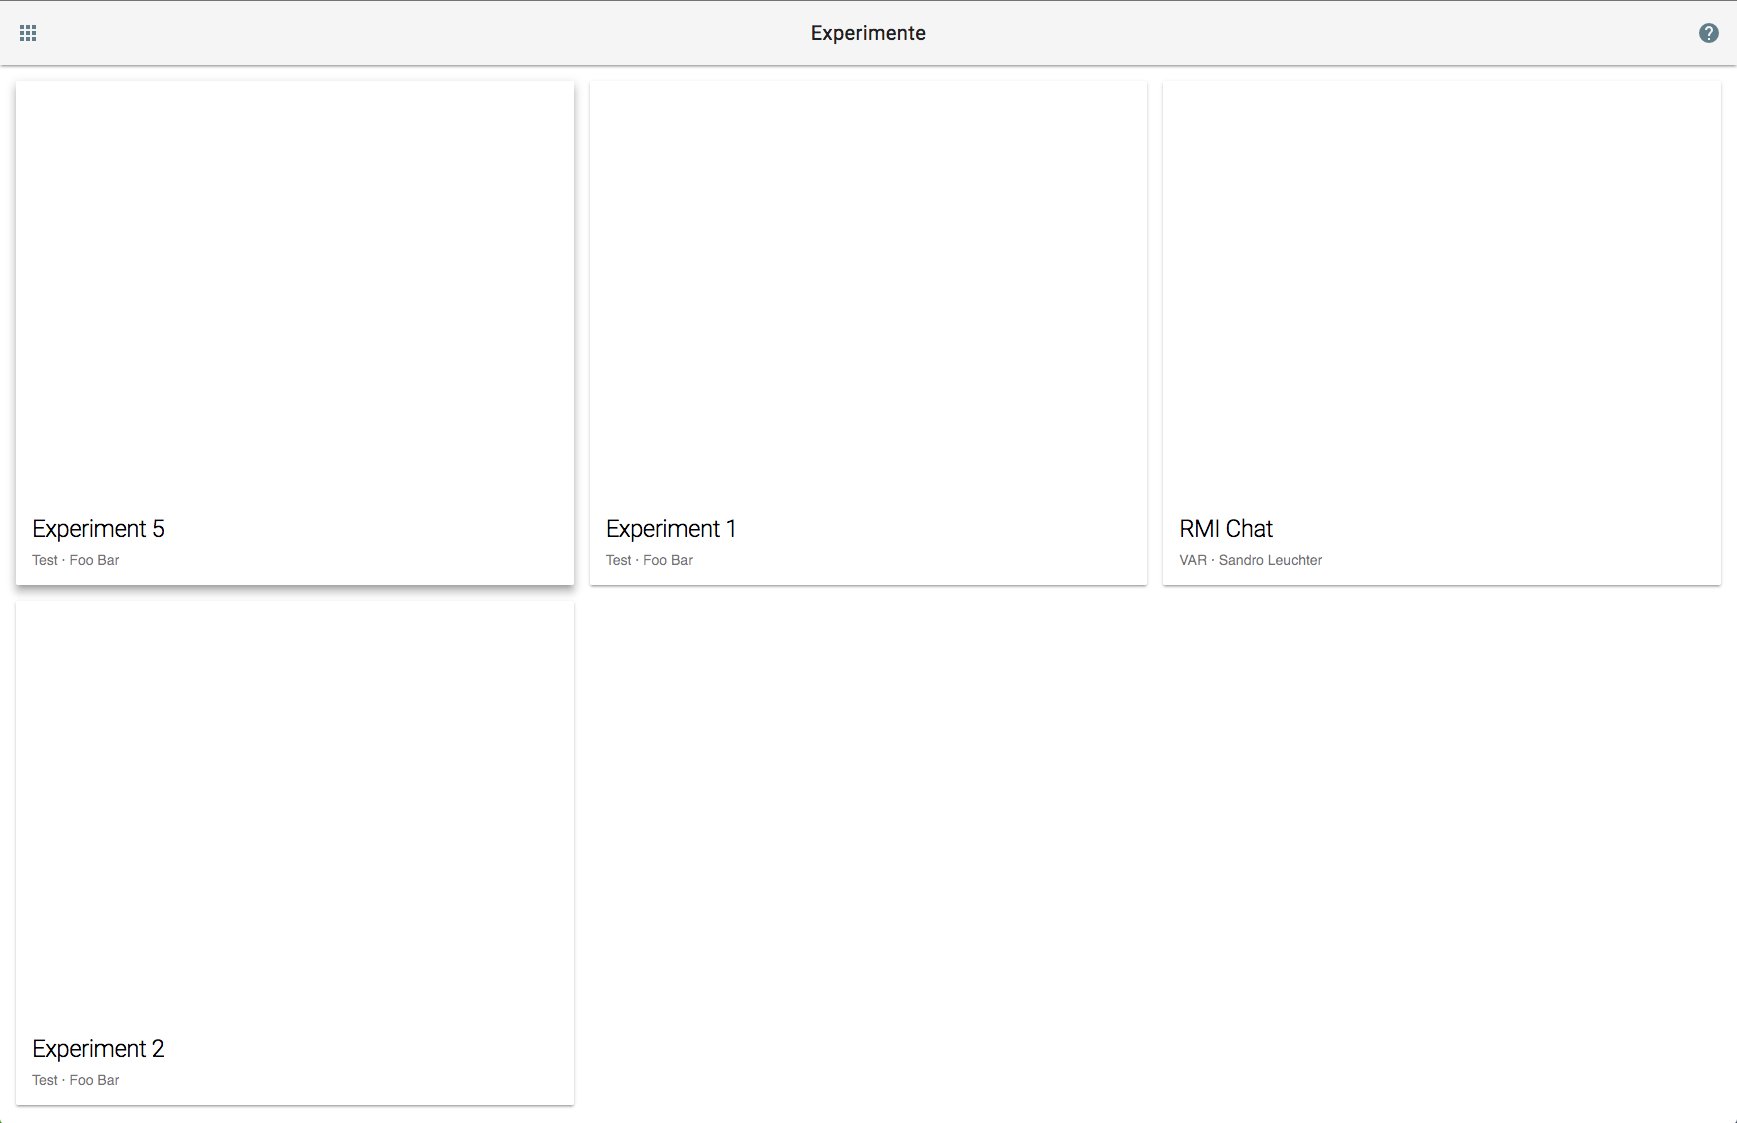
\includegraphics[scale=0.35]{current_dev_view_overview.png}}
    \par
    \caption{Umsetzung des Clients: Übersichtsseite}
    \label{fig:dev-view-1}
  \end{figure}
  \begin{figure}[h]
    \centering
    \fbox{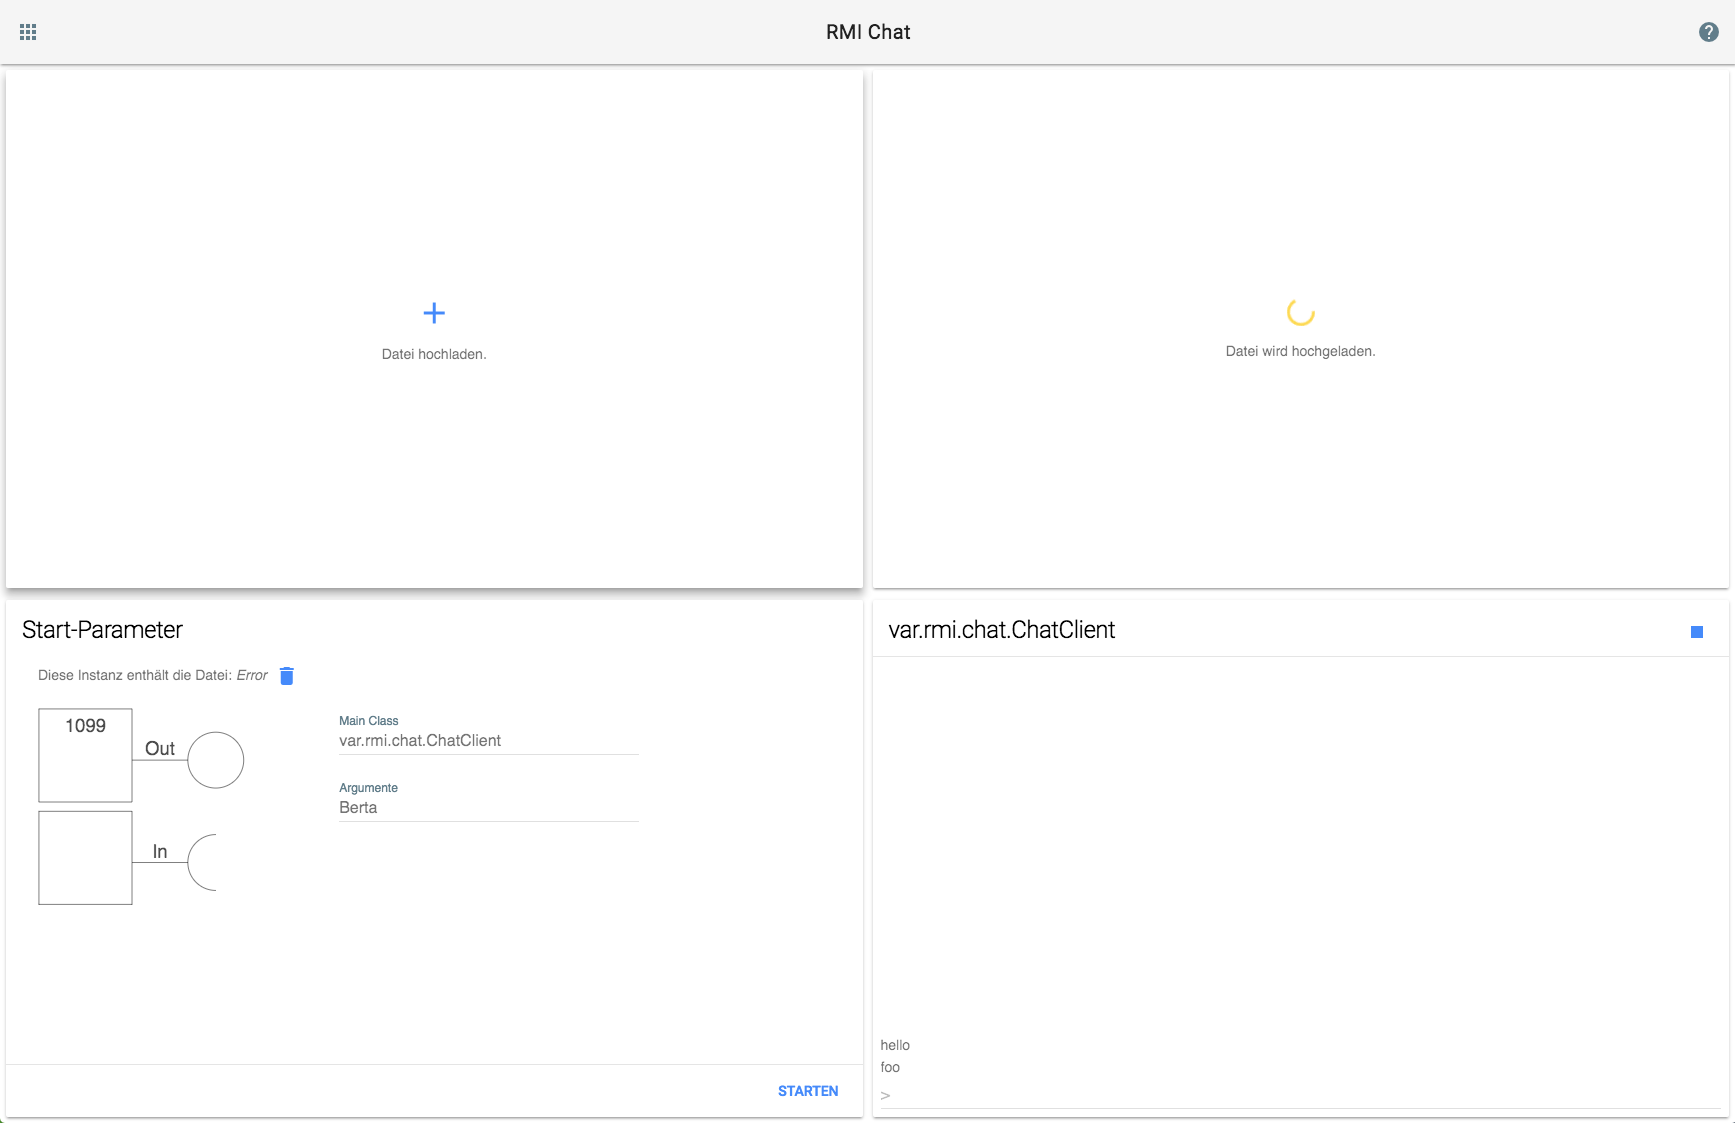
\includegraphics[scale=0.35]{current_dev_view_experiment.png}}
    \par
    \caption{Umsetzung des Clients: Experimentenansicht}
    \label{fig:dev-view-2}
  \end{figure}
\end{landscape}
\section{Erwartungen an die Performance}
Der Client ist über einen Websocket mit dem Server verbunden.
D.h. bei einer stabilen Internetverbindung sollten auftretende Logs innerhalb von wenigen Sekunden im Client sichtbar sein.
Dies ist möglich, da der Client nicht in einem bestimmten Interval nach neuen Logs frägt, sondern aktiv davon benachrichtigt wird.
\\
Auf Seiten der User-Container werden die Logs in eine Datei geschrieben und damit gepuffert.
Der Server wartet auf Änderungen an dieser Datei und gibt die Inhalte an den Client weiter.
Die Kopplung der User- und Server-Container über die Dateiebene sollte keine Performanceeinbußen bedeuten.
\par
Es wurden noch keine Leistungstests mit der Applikation gemacht, allerdings wäre es gerade in Hinblick auf einen Vergleich zu einem Deployment in einer herkömmlichen \ac{VM} sehr interessant durchzuführen.
Dies wäre bei einer Überführung des \texttt{docker-compose}-Files in ein \textit{Ansible}\footnote{\url{https://www.ansible.com/ansible-container}}-Playbook möglich, da man über dieses Tool mehrere Deployment-Targets nutzen kann.
Die damit erhaltene generalisierte Provisionierung der Instanz kann sowohl mit bspw. VMWare oder Docker genutzt werden.
\par
Wird die Applikation auf einem leistungsstarken Rechner ausgeführt, so sollten allerdings einige User-Container von den Studierenden gestartet werden können.
Sollte sich die Leistung eines Rechners dennoch als zu gering herausstellen, so könnte man die Applikation mit Docker Swarm oder Google Kubernetes über mehrere Hosts verteilen.
Es gibt dazu ein sehr breites Ökosystem mit Werkzeugen zu dieser Thematik.
\section{Installation}
Als erstes wird das Projekt mithilfe von \texttt{git clone \url{https://github.com/jwillem/var-tool.git}} heruntergeladen.
Um die Applikation zu starten, werden zunächst die Installationen von Docker\footnote{\url{https://www.docker.com/community-edition}} und Docker-Compose\footnote{\url{https://docs.docker.com/compose/install/}} benötigt.
Nach einem Ausführen von \texttt{docker-compose build} im Projektverzeichnis kann die App mit \texttt{docker-compose up} gestartet werden.
\\
Sollte eine weitere Entwicklung erfolgen, so können die vorbereiteten Development-Container genutzt werden.
Dazu führt man \texttt{docker-compose -f docker-compose\break .dev.yml up} aus.

  \chapter{Fazit}
Während der Entwicklung hatte sich herausgestellt, dass die eigentliche Überlegung, Apache Kafka für die Integration der einzelnen Services der Applikation zu nutzen, erheblich mehr Aufwand bedeutet hätte.
In der Vorbereitungsphase wurde eine Bibliothek Namens \textit{kafka-websocket} ausgewählt, welche es versprechen sollte, die Clients über Websocket an Kafka zu verbinden.
Bei näherer Betrachtung der Library wurde leider erkannt, dass das Format der einzelnen gesendeten Nachrichten an den sogenannten Kafka-Websocket-Proxy schwer zu verändern ist.
Dies passte jedoch nicht zu dem vorherig überlegten Nachrichten-Schema zur Kommunikation zwischen Server und Client.
Es wurde statt dem Einsatz von \textit{kafka-websocket} ein eigener Websocket-Endpoint im Server entwickelt, welcher das geplante Nachrichten-Schema umsetzt.
Die Übermittlung von Log-Daten aus den User-Containern in den Server wurde stattdessen über die Dateiebene des Docker-Hosts gestaltet.
Die User-Container schreiben eine \texttt{stdout}-Datei und lesen eine \texttt{stdin}-Datei um Eingaben zu akzeptieren.
Der Server liest die Datei \texttt{stdout} und gibt den Inhalt per Websocket an den Client weiter, bzw. schreibt in die Datei \texttt{stdin} um Eingaben vom Client an den Container weiterzugeben.
\par
Die Grundüberlegung bzw. in der Architektur\footnote{Hierzu kann im Repository des Projekts ein Diagramm mit dem Namen \texttt{deployment\_kafka.pdf} gefunden werden.} der Applikation Kafka einzusetzen, könnte in einer weiteren Arbeit erforscht werden.
Erzeugte Logs der User-Container könnten mit Kafka empfangen und auch persistent gespeichert werden.
So wäre es denkbar, dass die einzelnen Ergebnisse der Durchführungen der Experimente auch von einem Dozenten im Nachhinein betrachtet werden könnten.
Im Gesamten würde Kafka ebenso den Micro-Service Gedanke des Projekts weiter ausbauen.
\par
Die Verbindung zwischen Client und Server sollte in Zukunft nach aktuellen Best-Practices vorsorglich verschlüsselt werden.
Dazu kann für HTTPS ein SSL-Zertifikat von \ac{bspw.} \textit{let's encrypt}\footnote{\url{https://letsencrypt.org/}} genutzt werden.
Ebenso sollten die Websocket-Verbindungen mit TLS über WSS eingerichtet werden.
\par
Die geplante Abschottung der Container wurde bisher nur mit den Bordmitteln von Docker realisiert.
Diese ersetzen jedoch nicht den Einsatz von einzelnen Firewall-Rules mithilfe von \ac{bspw.} \textit{iptables}.
Bei einem tatsächlichen Deployment der Applikation könnte daher Server und Client über einen weiteren Proxy-Container (\textit{nginx}) geleitet werden, der außerdem eine Firewall implementiert.
\par
% \begin{itemize}
  % \item Umsetzung mit Kafka leider nicht m"oglich.
  % \item mehraufwand eigenen kafka proxy zu schreiben
  % \item grundüberlegung von kafka kann dennoch in folgenden arbeiten zu thema kommen
  % \item kafka kann log daten empfangen und auch dauerhaft vorhalten
  % \item microservice gedanke kann weiter ausgebaut werden
  % \item Ergebnisse (eigenes Kapitel?)
  % \item Performance!
  % \item websocket sollte über tls erfolgen
  % \item Im Experiment könnte noch bei geringem Aufand ein dnd-container zum einsatz kommen. 
  % \item Admin-Client muss noch in weiterer Arbeit entwickelt werden
  % \item Abschottung der Container muss noch mit bspw iptables geschehen
% \end{itemize}
\clearpage


  \pagenumbering{roman}
  \setcounter{page}{5}
  % \begin{appendices}
  \addcontentsline{toc}{chapter}{Quellenverzeichnis}
  \chapter*{Quellenverzeichnis}
  @book{Butcher:2014:SCM:2621977,
 author = {Butcher, Paul},
 title = {Seven Concurrency Models in Seven Weeks: When Threads Unravel},
 year = {2014},
 isbn = {1937785653, 9781937785659},
 edition = {1st},
 publisher = {Pragmatic Bookshelf},
}
\\
@book{tate2014seven,
  title={Seven More Languages in Seven Weeks: Languages that are Shaping the Future},
  author={Tate, B. and Dees, I. and Daoud, F. and Moffitt, J.},
  isbn={9781941222157},
  lccn={2015473679},
  series={Pragmatic programmers},
  url={https://books.google.de/books?id=lc-foAEACAAJ},
  year={2014},
  publisher={Pragmatic Bookshelf}
}
\\
@book{Higginbotham:2015:CBT:2836843,
 author = {Higginbotham, Daniel},
 title = {Clojure for the Brave and True: Learn the Ultimate Language and Become a Better Programmer},
 year = {2015},
 isbn = {1593275919, 9781593275914},
 edition = {1st},
 publisher = {No Starch Press},
 address = {San Francisco, CA, USA},
} 
  \clearpage

  \addcontentsline{toc}{chapter}{Abkürzungsverzeichnis}
  \chapter*{Abkürzungsverzeichnis}
\begin{acronym}
\acro{Abb.}{Abbildung}
 \acro{Abk.}{Abkürzung}
 \acro{AJAX}{Asynchronous Java-Script and XML}
 \acro{bspw.}{beispielsweise}
 \acro{bzw.}{beziehungsweise}
 \acro{EVA}{Eingabe, Verarbeitung, Ausgabe}
 \acro{VAR}{Verteilte Architekturen}
 \acro{VM}{Virtuelle Maschine}
 \acrodefplural{VM}[VM's]{Virtuelle Maschinen}
 \acro{IDE}{Integrated-Development-Environment}
 \acrodefplural{IDE}[IDE's]{Integrated-Development-Environments}
 \acro{SPA}{Single-Page-Application}
 \acrodefplural{SPA}[SPA's]{Single-Page-Applications}
 \acro{RIA}{Rich-Internet-Application}
 \acro{REST}{Representational state transfer}
 \acrodefplural{RIA}[RIA's]{Rich-Internet-Applications}
 \acro{TCP}{Transmission Control Protocol}
 \acro{u.A.}{unter Anderem}
 \acro{z.B.}{zum Beispiel}
\end{acronym}

  % \end{appendices}

\end{document}
